%!TEX root = Vorlage_Buch.tex

\chapter{Tierisch Gutes}\label{Chapter2}
\lettrine[lines=3]{I}{n diesem Kapitel} beschäftigen wir uns mit Fleisch, Fisch 
und Geflügel, das auf den Grill zubereitet wird.  
Genauso vielfältig wie die Grill-Geräte sind die Rezepte die auf den Grills 
zubereitet werden. Für jede Art von Grill gibt es 
Rezepte die dafür wie geschaffen sind.

\section{Rind}

Die große Auswahl an Fleischrinderrassen bietet letztendlich für jeden 
Geldbeutel und Geschmack das richtige Fleisch. 

\begin{description}
	\item[Aberdeen Angus] Weltweit verbreitet, schön mamoriertes, 
	aromatisches Fleisch
	\item[Brangus] Kombinationsrasse aus Brahman und Angus, beliebt in 
	Südamerika, Australien und Asien, schön mamoriertes, aromatisches 
	Fleisch
	\item[Charolais] ist ein französisches Rind, das wegen seinem 
	mageren, mit feinen Fettadern durchzogenem Fleisch bei Kennern sehr 
	beliebt ist
	\item[Chianina] Eine der ältesten und die größte Rinderrasse der Welt. 
	Das magere Fleisch schmeckt unvergleichlich zart und würzig.
	\item[Deutsch Angus] Ist für die Freilandhaltung gut geeignet. Das 
	Fleisch ist besonders schmackhaft durch die feinen Fleischfasern und 
	die gute Mamorierung.
	\item[Galloway] Ursprung südwestliches Schottland, kommt gut mit 
	Trockenheit, Kälte und Schnee zurecht. Das saftige, aromatische 
	Fleisch ist gut mamoriert und weist eine leichte Wildnote auf.
	\item [Das ursprünglich aus England stammende Hereford-Rind] passt 
	sich an jedes Klima an und ist somit weltweit vertreten. Das Fleisch 
	zeichnet sich durch intensiven Geschmack und eine feine Mamorierung 
	aus.
	\item [Das Heckrind] wurde in 1930er Jahren von den Gebrüdern Heck 
	gezüchtet. Sie kreuzten 8 Wildrassen und 17 Hausrassen mit dem Ziel, den 
	Auerochsen wieder aufleben zulassen, der im 17ten Jahrhundert 
	ausgestorben ist. Das Ziel wurde nicht erreicht, heraus kam allerdings ein 
	robustes, krankheitsresistentes Rind, das ganzjährig auf der Weide steht da 
	es sehr temperaturtolerant ist. Das Fleisch hat einen intensiven Geschmack 
	und ist durch die kurzen Fleischfasern sehr zart und reich an Vitaminen und 
	Omega-3-Fettsäuren.
	\item[Das Hinterwälder Rind] kommt aus dem Schwarzwald und ist fast 
	ausgestorben. Nur der Initiative einer weniger Landwirten ist der 
	Fortbestand zu verdanken. Das Fleisch ist sehr selten und zeichnet 
	sich durch eine feine Faser mit solider Fetteinlagerung aus. Durch die 
	natürliche Fütterung mit Gras und Heu prägt sich ein mineralisch 
	-intensiver Geschmack aus.
	\item[Kobe-Rinder] kommen aus der japanischen Präfektur Hyogo mit 
	dem Verwaltungssitz Kobe. Die Rasse nennt sich Tajima, im Westen 
	allerdings Wagyu. Das Fleisch der Kobe-Rinder ist extrem Fett, das 
	zeigt sich an der hellroten bis rosa-roten Farbe, der Fleischgeschmack 
	ist sehr mild. Das Fleisch hat allerdings einen schönen Schmelz.
	\item[Limousin-Rinder] stammen aus der gleichnamigen Region in 
	Frankreich. Durch die zarte Faserung und das optimale 
	Fleisch-Fett-Verhältnis ist das Fleisch saftig und sehr zart.
	\item [Pinzgauer Rinder] haben eine dunkle Fleischfarbe, eine sehr 
	feine Verteilung des Fetts im Fleisch und ein stark mineralisches 
	Aroma, da die Tiere fast ausschließlich aus Weidehaltung stammen.
	\item [Rubia Gallega oder auch Galicisches Blondvieh] ist eine alte 
	spanische Hausrinderrasse aus Galizien. Genießer schätzen vor allem 
	die dunkle Fleischfarbe, die ausgeprägte Fettmarmorierung und das 
	intensiv-kräftige Aroma.
	\item [Schottische Highlands] leben das ganze Jahr im Freien und 
	werden gerne zu Landschaftspflege eingesetzt. Das Fleisch ist 
	kurzfaserig und dadurch zart und saftig.
	\item[Shorthorns] sind kleine englische Rinder, die rasch 
	ausgewachsen sind und dann zur Verfettung neigen. Das heißt, die 
	Energie im Futter wird in Form von Fett in den Muskel eingelagert. Das 
	sorgt für einen zarten und saftigen Schmelz.
	\item[Simmentaler Rind] kommt aus dem gleichnamigen Simmental im 
	Berner Oberland. In Deutschland und Österreich gehören sie zu dem 
	bedeutendsten Rinderrassen. Gourmets schätzen den aromatischen 
	Geschmack und die feine Mamorierung.
	\item[Das Wagyu-Rind] hat die höchste Fettmamorierung aller 
	Rinderrasen, welche für die Saftigkeit und Zartheit diese Fleisches 
	verantwortlich ist. Siehe auch Kobe-Rind.
\end{description}

\subsection{Roastbeef vom Keramikgrill}
Roastbeef ist ein besonders zartes und saftiges Stück Fleisch, das aus 
dem hinteren Rücken des Rindes stammt. Es ist bekannt für seine feine 
Marmorierung und wird oft im Ganzen zubereitet. Traditionell wird es in 
Großbritannien als klassisches Sonntagsessen serviert. 

\paragraph{Geräte}

\begin{itemize}[noitemsep]
	\item Kamado Grill (Keramikgrill)
\end{itemize}


Vorbereitung des Kamado Grills: Der Feuerkorb wird abgeteilt und eine Hälfte
mit Holzkohlen gefüllt. Die Seite auf mit der 
Holzkohle für direkte Hitze
vorbereiten. Das heißt eine Hälfte des Grillrosts auf die unterste Stufe 
über die Holzkohle legen. Die andere Seite für indirekte Hitze vorbereiten. 
Einen halben Deflektorstein neben den Grillroast auf die unterste Stufe 
legen. Eine Hälfte der Fettauffangschale auf den Deflektorstein stellen 
und die zweite Rosthälfte auf die oberstes Stufe legen. Den Grill anheizen 
und die Temperatur auf 150℃ einstellen. Die Temperatur wird im Dom 
gemessen
und ist daher niedriger als direkt über den Kohlen. Diesen Umstand 
machen
wir uns zu Nutze, in dem wir das Roastbeef in der indirekten Zone auf den
gewünschten Gargrad ziehen. Bei einem Roastbeef ist meines Erachtens
eine Temperatur 55℃ bis 57℃ (medium rare bis medium) mit einer 
Tendenz
zu 57℃ anzustreben, da die meisten Menschen medium gegartes Fleisch
bevorzugen.

\paragraph{Zutaten}

\begin{itemize}[noitemsep]
	\item Roastbeef (ca. 1,5 kg)
	\item 10 g/ kg Fleisch grobes Himalaya-Salz
	\item 5 g bis 7 g schwarzer Pfeffer (hier Whisky-Pfeffer), ganze Körner 
	im Mörser zerkleinert
\end{itemize}

\paragraph{Zubereitung}

Salz und Pfeffer mischen. Das Roastbeef von allen Seiten gleichmäßig mit 
der Salz-Pfeffermischung würzen und diese leicht einmassieren. Danach
das Roastbeef auf der direkten Hitze von allen Seiten angrillen, bis die
Oberfläche karamellisiert und sich Röststoffe gebildet haben. Wenn das
Fleisch auf allen Seiten angeröstet ist, wird es auf die indirekte Hitze 
gelegt
und auf die gewünschte Temperatur hochgezogen. Das Fleisch bei 
erreichen
der Temperatur vom Grill nehmen und in Butterbrotpapier oder besser in
Butchers paper einwickeln und für 10 bis 20 Minuten in einer 
Warmhaltebox
ruhen lassen. Das Fleisch im dünne Scheiben schneiden und servieren, 
siehe Abbildung~\vref{fig:Roastbeef}
Dazu Beilagen nach Wahl reichen.

Alternativ kann das Roastbeef auf dem Kugelgrill zubereitet werden. Dazu
muss der Kugelgrill mit der Zwei-Zonen-Glut (siehe Kapitel~\ref{Chapter1} 
\vref{fig:ZweiZonen}) vorbereitet werden. Auf dem
Gasgrill wird die Temperatur mit einem oder zwei Brennern eingestellt und
das Fleisch auf der direkten Hitze angegrillt.
\newpage
\begin{figure}[htbp]
	\centering
	\begin{minipage}{1\textwidth}
		\centering
		\includegraphics[width=1\linewidth]{pics/Roastbeef_2}
		\captionof{figure}{Roastbeef vom Keramikgrill}
		\label{fig:Roastbeef}
	\end{minipage}
\end{figure}
\newpage

\subsection{Roastbeef unter der Kräuterkruste}

\paragraph{Geräte}

\begin{itemize}[noitemsep]
	\item Napoleon Gasgrill Rogue 425
\end{itemize}

\paragraph{Zutaten}

Für das Roastbeef:

\begin{itemize}[noitemsep]
	\item Roastbeef (ca. 1,5 kg) 
	\item 100 g Semmelbrösel
	\item 100 g weiche Butter
	\item 2 TL körniger Senf
	\item 2 EL Olivenöl
	\item Salz  \& Pfeffer
	\item 2 Zweige Rosmarin
	\item 2 Knoblauchzehen
\end{itemize}

Für die Soße:

\begin{itemize}[noitemsep]
\item 1 Karotte
\item 1 Zwiebel
\item 50 g Lauch
\item 1 Knoblauchzehe
\item 1 EL Tomatenmark
\item 1 TL Paprikapulver
\item 1 TL Mehl
\item 300 ml Schwarzbier (bei Köstritzer Schwarzbier)
\item 300 ml Rinderfond
\end{itemize}
\newpage

\paragraph{Zubereitung}

Die Zubereitung des Roastbeefs erfolgt im Gasgrill. Alternativ kann das
Gericht auch im Backofen zubereitet werden. 

Den Gasgrill auf ca. 230℃ 
bis 260℃ aufheizen und das Roastbeef von allen Seiten scharf anbraten. Das 
Fleisch zur Seite legen damit es Temperatur verliert, so lässt die Kräuterkruste 
besser aufbringen, da die Butter bei zu hoher Temperatur schnell schmilzt.

Während das Fleisch und der Grill abkühlen, widmen wir uns der Kräuterkruste. 
Dafür werden alle Zutaten in einer Schüssel vermengt und 
verrührt.
Wenn alles ordentlich vermengt ist, wird die Kruste gleichmäßig auf das
Fleisch verteilt.

Bevor das Fleisch jetzt zum Garen auf den Grill gestellt wird, muss
die Soße zubereitet werden. Eine Gusseiserne Pfanne auf dem 
Seitenkochfeld
des Gasgrills erhitzen und das Gemüse in der Pfanne angebraten. Wenn 
das
Gemüse angebraten ist und die Zwiebeln glasig sind, kommen Mehl,
Paprikapulver und das Tomatenmark dazu und werden kurz mit 
angebraten.
Anschließend wird alles mit dem Schwarzbier abgelöscht und mit dem
Rinderfond aufgefüllt und 2 bis 3 Minuten gekocht.

Jetzt wird das Fleisch mit der vorher aufgetragenen Kruste nach oben in
die Soße gelegt, ein Kerntemperaturfühler in das Fleisch eingesteckt und in den 
vorgeheizten Grill gestellt.
Kurz bevor das Fleisch die gewünschte Kerntemperatur (ich empfehle 55°C bis 
57°C) erreicht hat, wird
der Heckbrenner des Grills angestellt und auf die höchste Stufe 
eingestellt, damit die Kruste kross wird und eine schöne Farbe bekommt. 
Aufpassen!
Das geht sehr schnell.

\begin{figure}[htbp]
	\centering
	\begin{minipage}{1\textwidth}
		\centering
		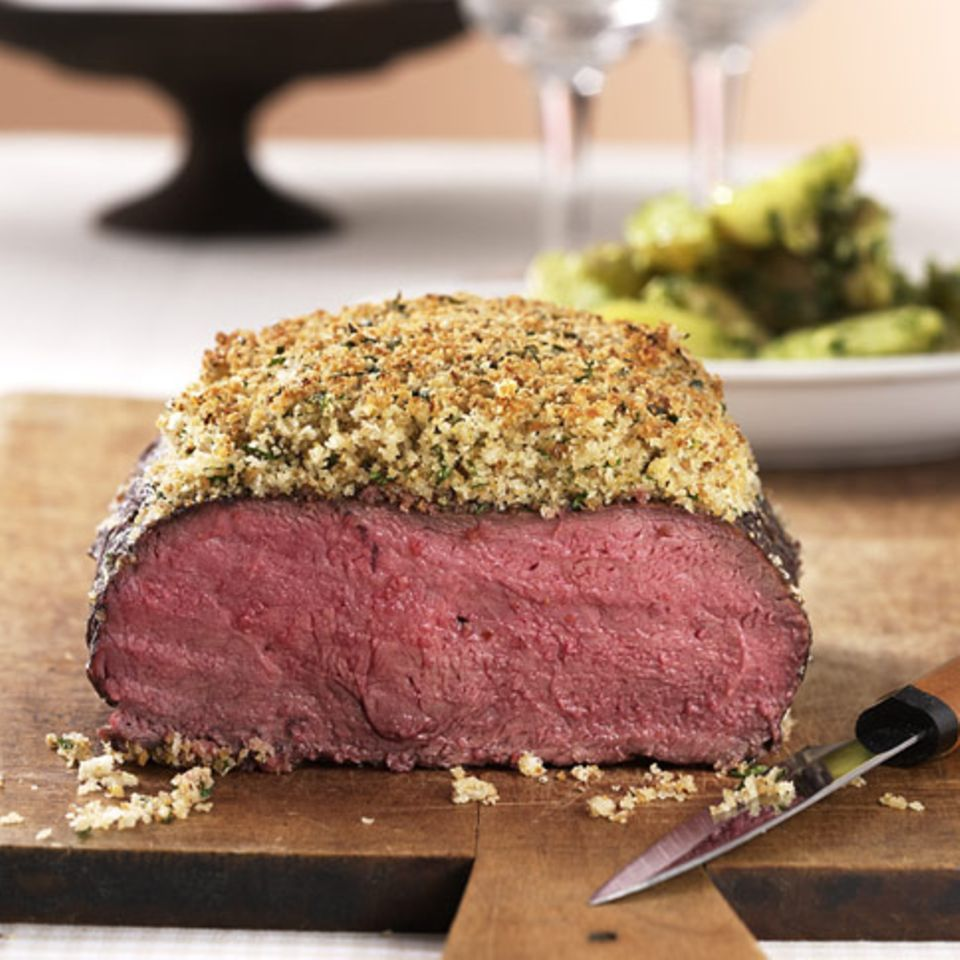
\includegraphics[width=1\linewidth]{pics/roastbeefmitkraeuterkruste}
		\captionof{figure}{Roastbeef vom Keramikgrill}
		\label{fig:Roastbeef}
	\end{minipage}
\end{figure}
\newpage

%\begin{figure}[htbp]
%	\centering
%	\begin{minipage}{1\textwidth}
%		\centering
%		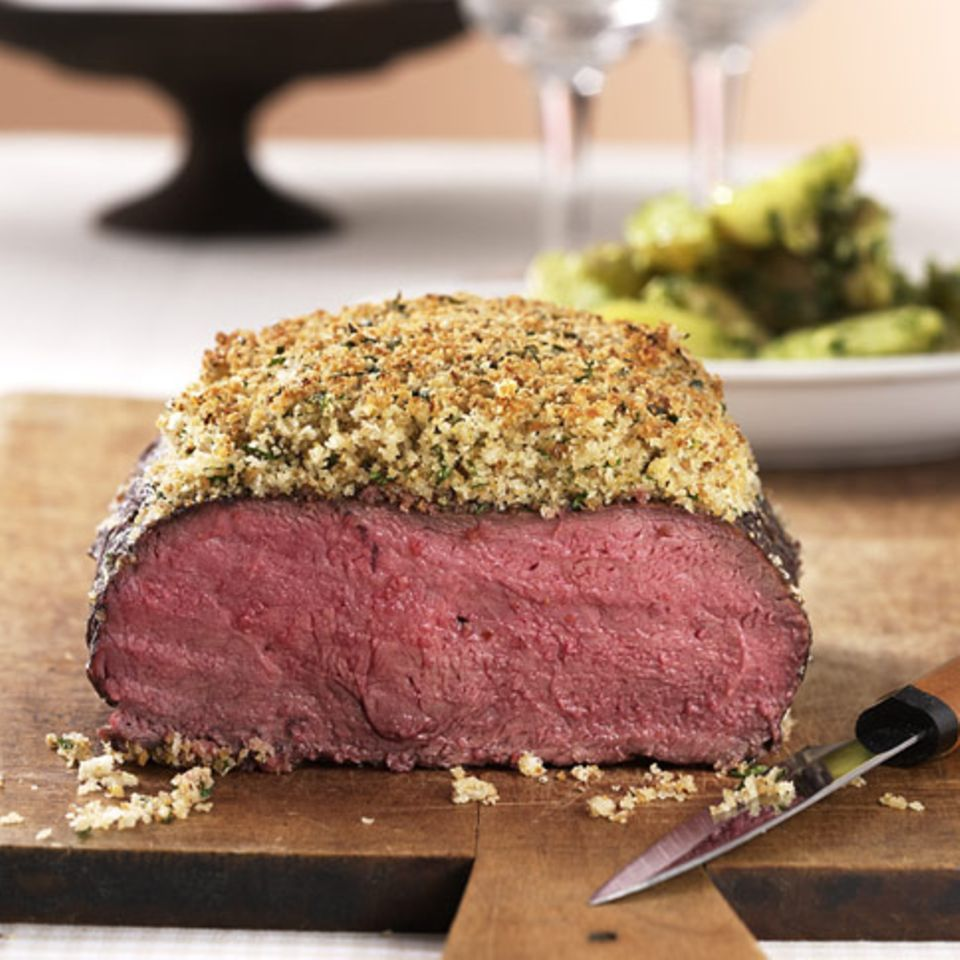
\includegraphics[width=1\linewidth]{pics/roastbeefmitkraeuterkruste}
%		\captionof{figure}{Roastbeef mit Kräuterkruste vom Gasgrill}
%		\label{fig:Roastbeef}
%	\end{minipage}
%\end{figure}
%\newpage

\subsection{Beef brisket}

\paragraph{Geräte}

\begin{itemize}[noitemsep]
	\item Water smoker
\end{itemize}

\paragraph{Zutaten}

\begin{itemize}[noitemsep]
	\item 1 Rinderbrust full packer von der Simmentaler Färse (Brust bestehend aus Flat and point, pariert ca. 5,5 bis 6,0 kg)
	\item grobes Salz (hier Himalaya-Salz, ca. 9 g/ kg Fleisch)
	\item schwarzer Pfeffer, ganz (ich verwende Telly Cherry Pfeffer, ca. 9 g/ kg Fleisch)
	\item Rauch (ich verwende Apple Wood Chuncks)	
\end{itemize}

\paragraph{Zubereitung}

Den Water Smoker vorbereiten und eine Temperatur von 135°C bis 140°C anvisieren.
Die Rinderbrust parieren, d. h. überflüssiges Fett entfernen, die Kanten rund schneiden, 
lose Enden sollten entfernt werden. Das Brisket mit dem Rub großzügig und gleichmäßig 
einreiben, wer mag kann noch etwas Zwiebel- und Knoblauchpulver zu der 
Salz-Pfeffermischung geben. Das Fleisch auf den oberen Rost legen und den Deckel 
wieder schließen. Apple Wood Chuncks auf die Holzkohle legen, so dass Rauch für ca. 1 
Stunde entsteht. Das Fleisch von Zeit zu Zeit mit etwas Flüssigkeit besprühen, damit die 
dünnen Enden nicht zu stark bräunen. Sobald das Fleisch eine gute Farbe hat, nach ca. 
2,5 bis 3 Stunden, in Butchers paper mit etwas Rinderfond, Apfelsaft oder Wasser einschlagen
und solange weiter garen bis eine Kerntemperatur von 95°C erreicht wird. Wichtiger als 
die Temperatur ist allerdings ein widerstandsloses eindringen des Messfühlers. Sobald 
noch ein spürbarer Widerstand zu fühlen ist, ist das Brisket noch nicht fertig. 

Wenn das Brisket fertig gegart ist, noch eingepackt in eine Thermobox oder Styroporbox 
legen und eine halbe bis eine Stunde ruhen lassen. Danach das Brisket (siehe siehe Abbildung~\vref{fig:Brisket}) mit Coleslaw
 (Rezept siehe Kapitel~\ref{Chapter5} \vref{Coleslaw}) und beliebigen Beilagen servieren.

\begin{figure}[htbp]
	\centering
	\begin{minipage}{1\textwidth}
		\centering
		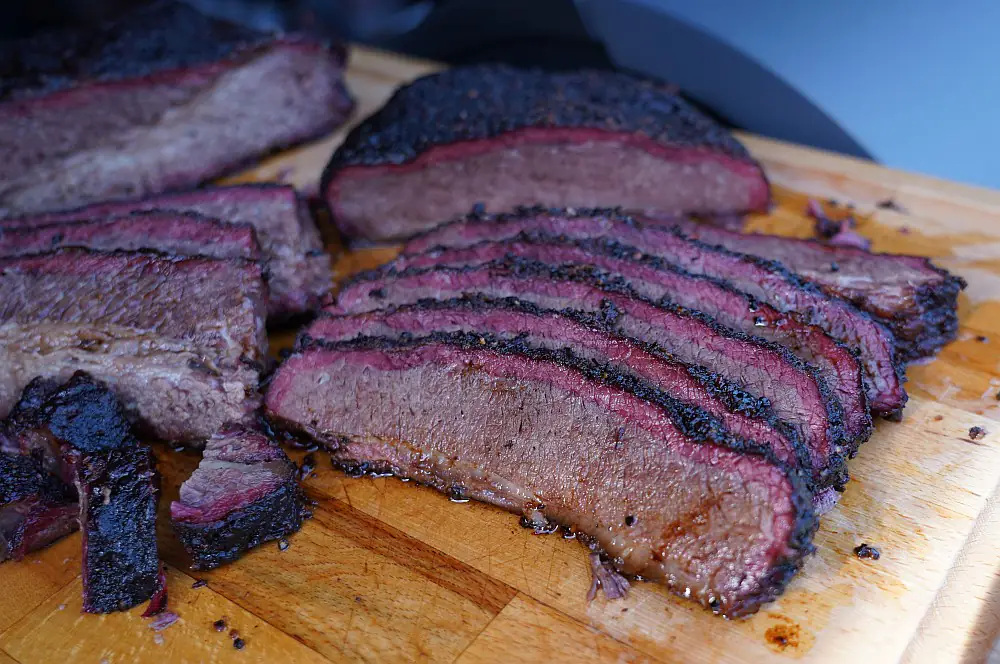
\includegraphics[width=.9\linewidth]{pics/Brisket}
		\captionof{figure}{Beef Brisket vom Water Smoker}
		\label{fig:Brisket}
	\end{minipage}
\end{figure}
\newpage

\subsection{Tomahawk Steak}

\paragraph{Geräte}

\begin{itemize}[noitemsep]
	\item Oberflächengrill Beefbox
	\item Keramikgrill
\end{itemize}

\paragraph{Zutaten für 2 Personen}

\begin{itemize}[noitemsep]
	\item 1 Tomahawk Steak (ca. 1,1 kg zur Metzgers Freude kann es auch ein 
	wenig mehr sein)
	\item Salz (ich benutze Himalaya-Salz aus der Mühle)
\end{itemize}

\paragraph{Zubereitung}

Den Keramikgrill hoch heizen und die Temperatur auf 150°C einstellen.
Das Steak in der Beefbox von jeder Seite ca. 1 Minute und 30 Sekunden scharf 
angrillen, evtl. kann es länger gehen bis das Fleisch schön karamellisiert ist.
Das angegrillte Steak auf dem Keramikgrill je nach Geschmack garziehen siehe 
Abbildung~\vref{fig:Toma2}. Auf einem Holzbrett anrichten in Tranchen 
schneiden und servieren.
Dazu den Eisbergsalat mit Champignons und Tomatendressing reichen.
Ich bevorzuge dazu einen schönen Shiraz, z.B. Fat Baron 2022.
\newpage
\begin{figure}[htbp]
	\centering
	\begin{minipage}{1\textwidth}
	\centering	
	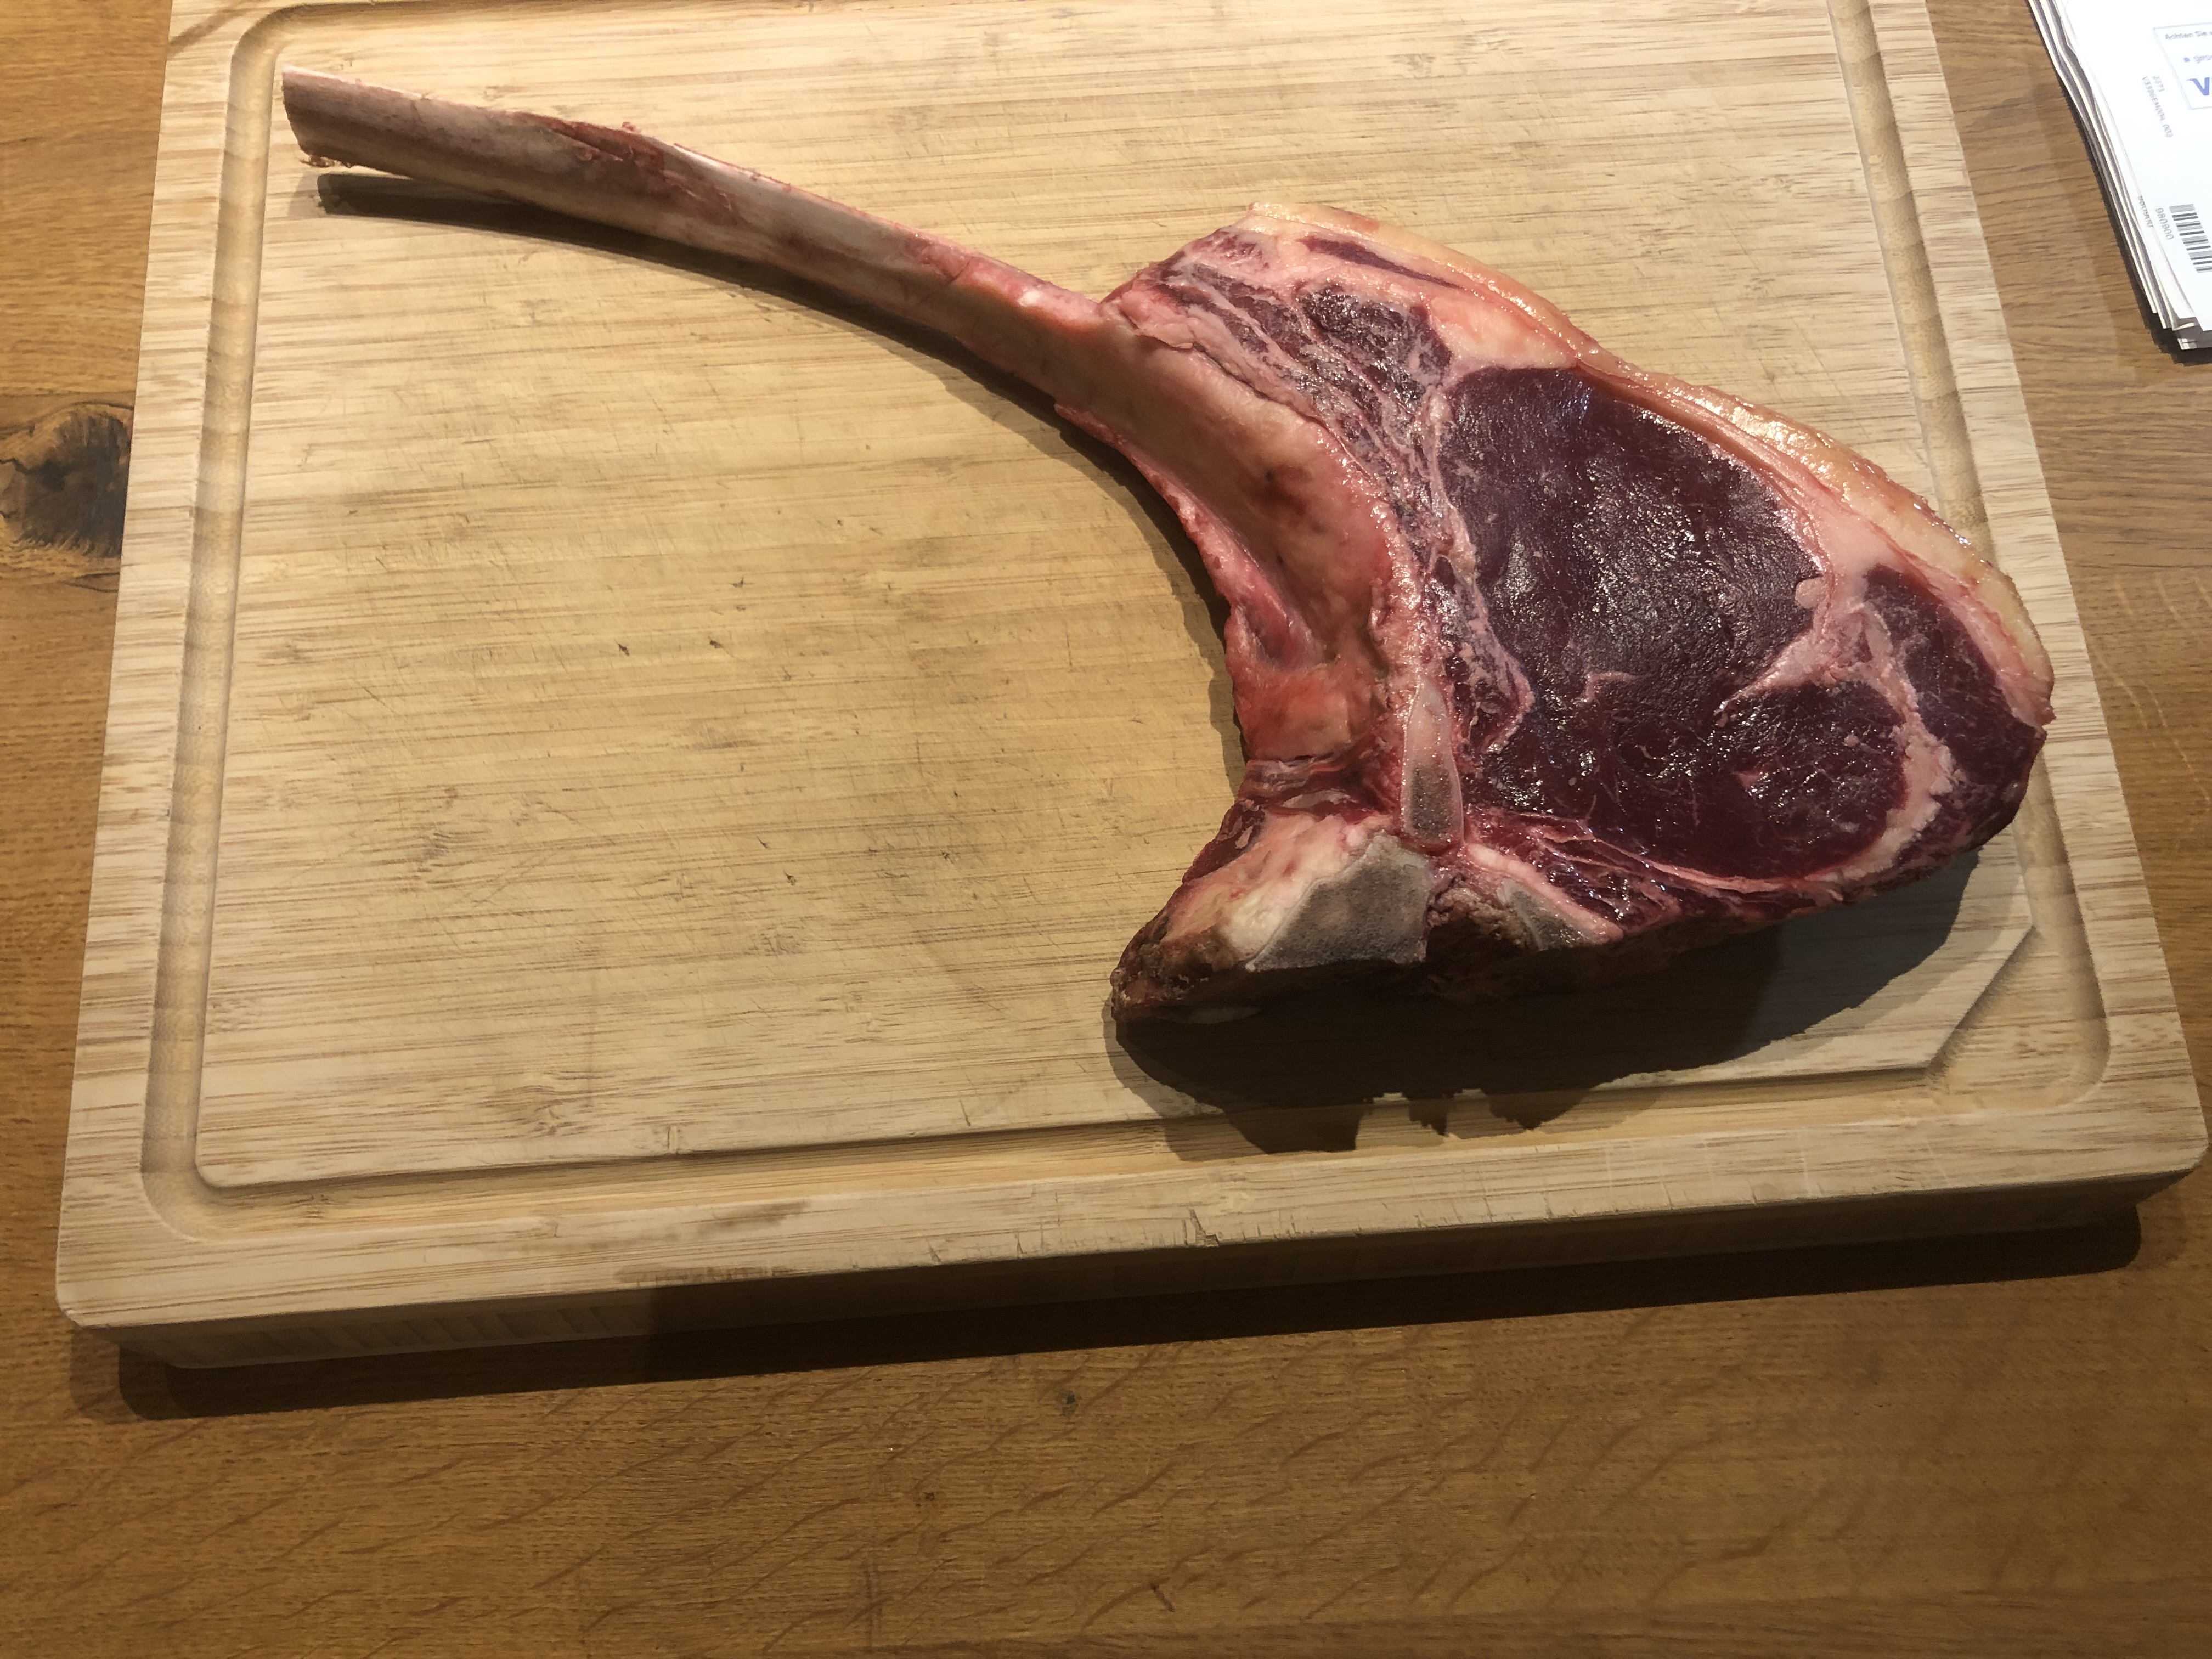
\includegraphics[width=1\linewidth]{pics/Tomahawk_roh}
	\captionof{figure}{Tomahawk Steak vor dem Grillen}
	\label{fig:Toma1}
	\end{minipage}
\end{figure}

\begin{figure}[htbp]
	\centering
	\begin{minipage}{1\textwidth}
	\centering
	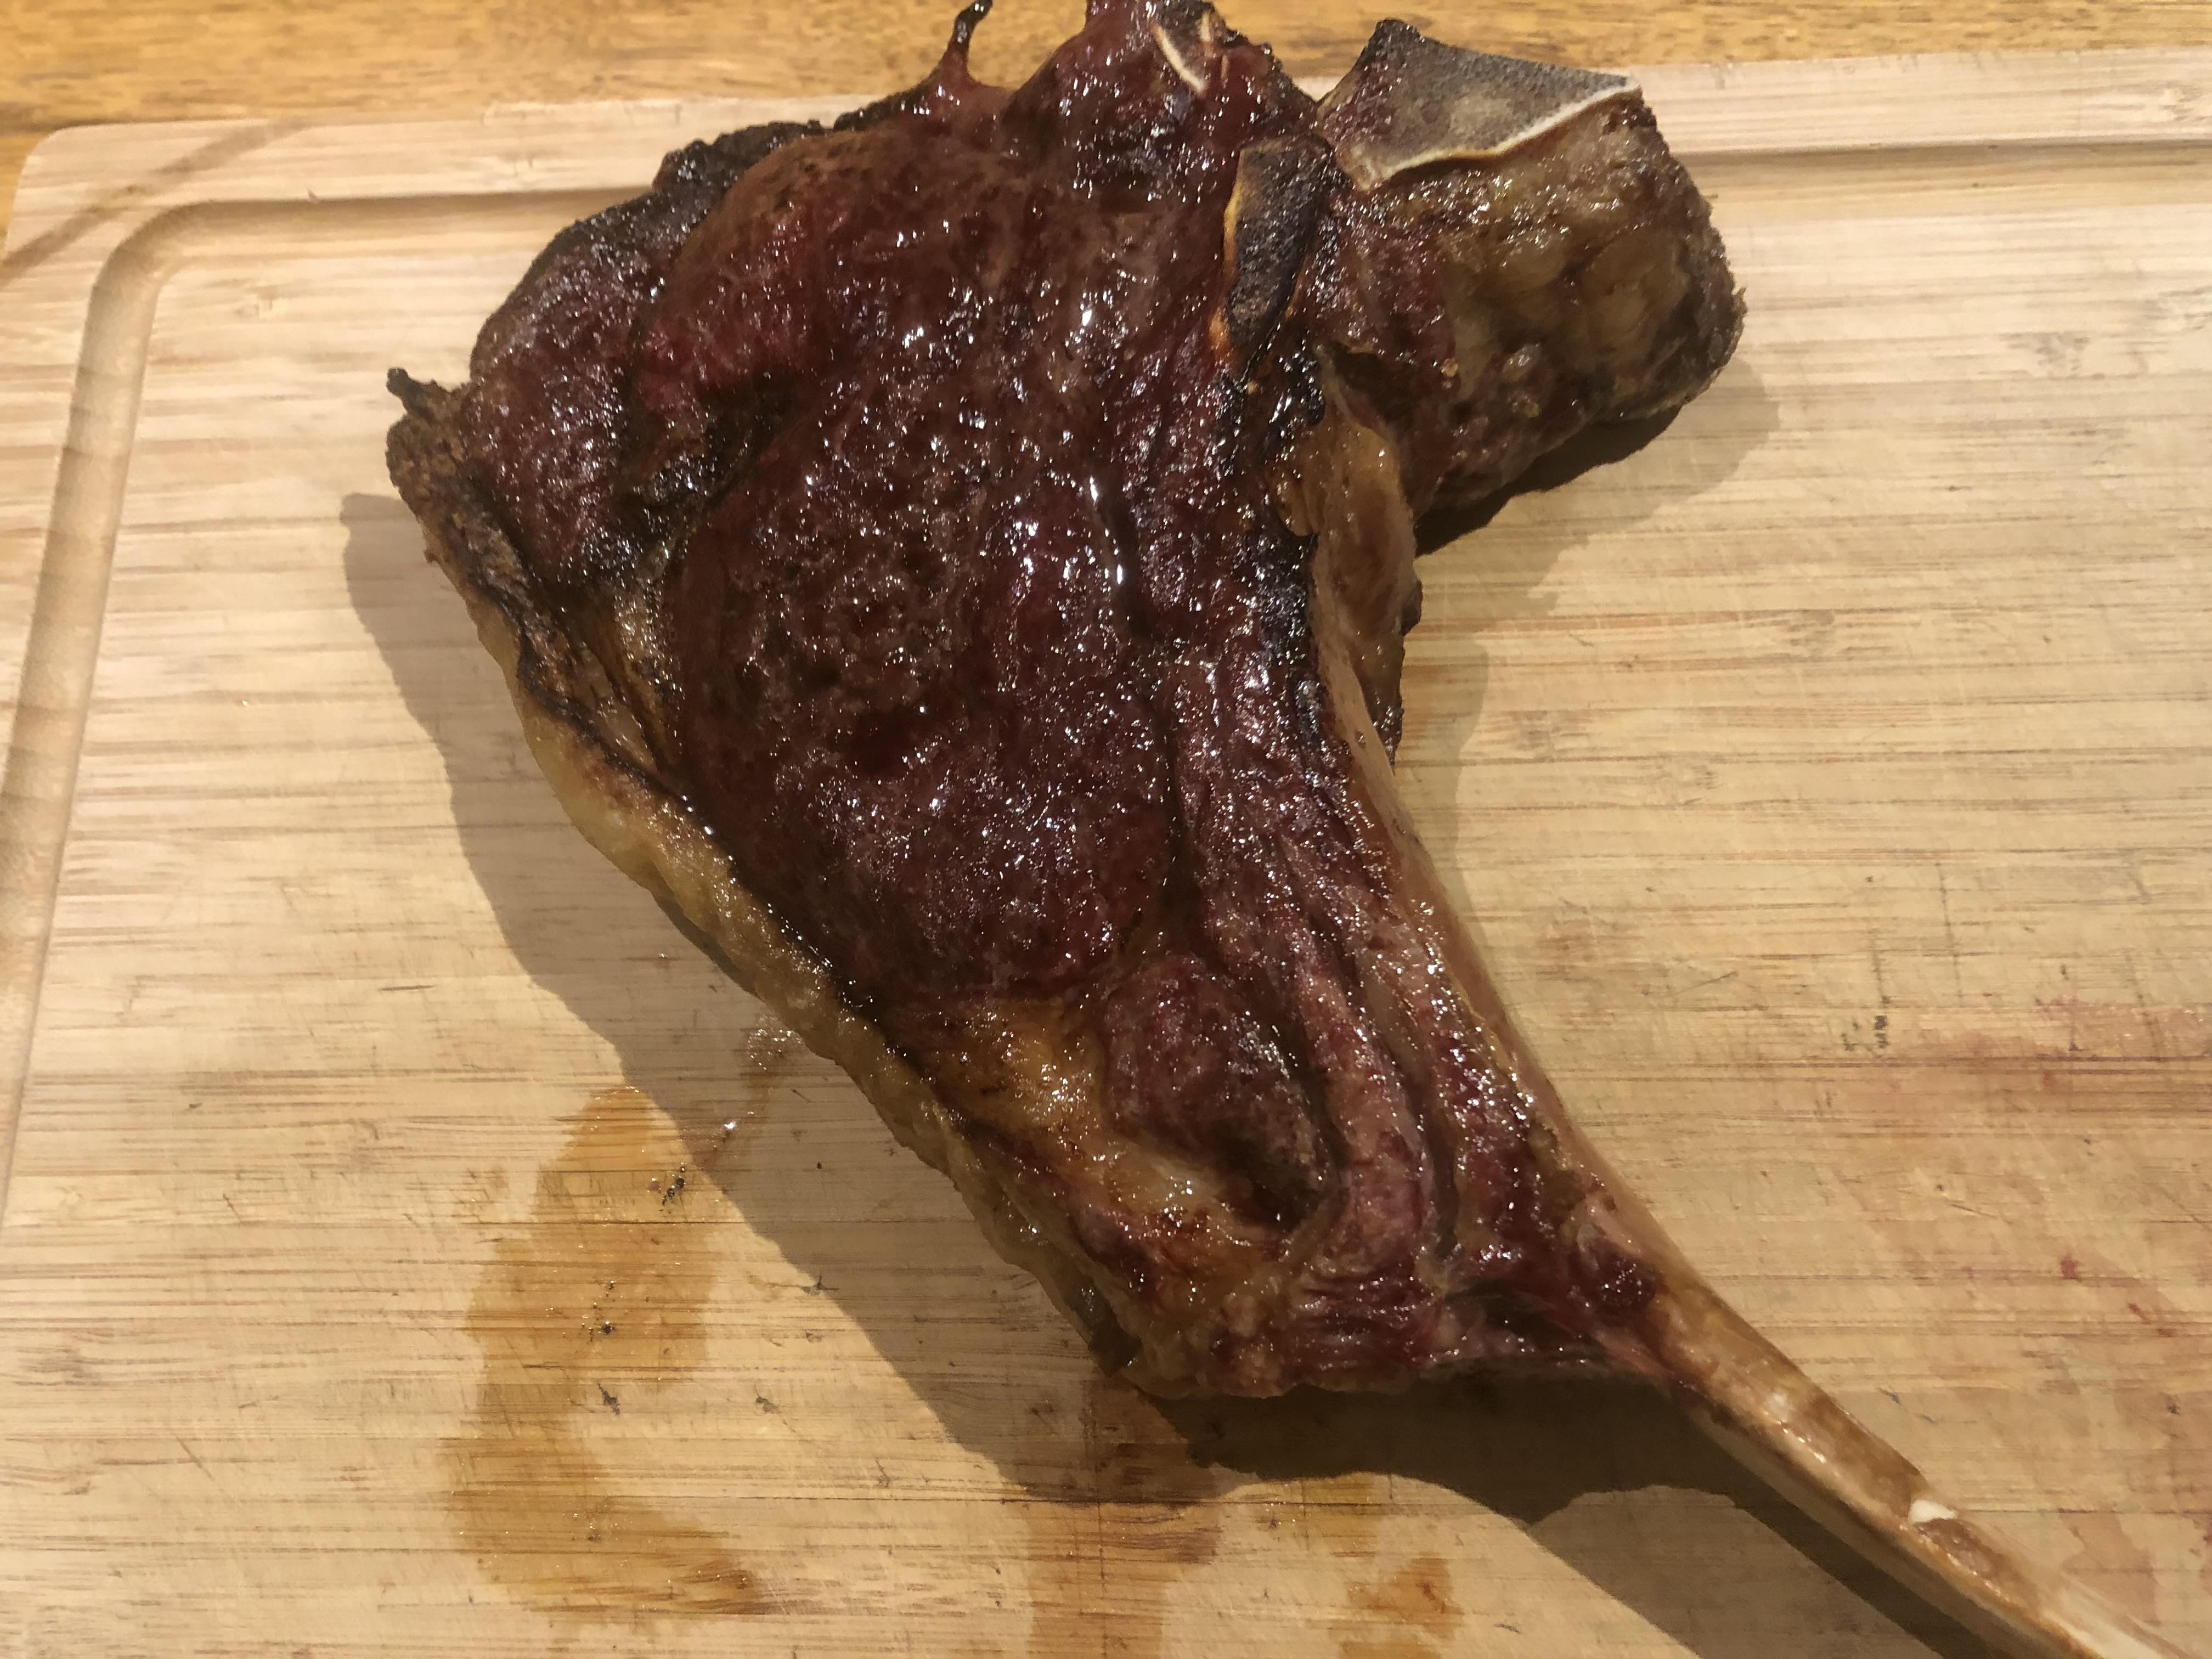
\includegraphics[width=.9\linewidth]{pics/Tomahawk_gegrillt}
	\captionof{figure}{Tomahawk Steak}
	\label{fig:Toma2}
	\end{minipage}
\end{figure}
\newpage

\subsection{Chili con carne}
Die Staaten Texas, New Mexico und Arizona erheben Anspruch auf den Ursprung des Chili con carne. Es gibt viele Geschichten über das Urrezept. Unbestritten ist jedoch 
der mexikanische Einfluss, in der mexikanischen Küche werden verschiedene 
Chilisorten eingesetzt um den Geschmack zu variieren.

Hier werde ich zwei Rezepte vorstellen, ein schwarzes, schweres Chili das 
eher in die Wintermonate passt und ein leichtes helles Chili Rezept 
siehe~\vref{Helles Chili}, das perfekt für die Sommermonate ist.

\subsubsection{Schwarzes Chili}
Dieses schwarze Chili ist sehr schwer und mit seinem Gewürzen eher für die 
kalten Herbst- und Wintermonate geeignet. Die schärfe des Chilis ist wie ein 
innerer Ofen und sorgt für eine angenehme Wärme.

\paragraph{Geräte}

\begin{itemize}[noitemsep]
	\item Dutch oven
\end{itemize}

\paragraph{Zutaten Chili}

\begin{itemize}[noitemsep]
	\item 1 große Zwiebel(n), rot
	\item 2 Knoblauchzehe(n)
	\item 500 g Hackfleisch, vom Rind
	\item 1 Dose/n Tomate(n) (400 g)
	\item 2 Dose/n Bohnen, schwarz (400 g)
	\item 2 cl Whisky (Bei mir 10 Jahre alter Laphroig von der Isle of Islay, einer 
	der rauchigsten Whiskys der Welt)
	\item 200 ml Bier (Bei mir Köstritzer Schwarzbier)
	\item 100 ml Kaffee (Bei mir 2 Espressi à 50 ml)
	\item 1 EL	Tomatenmark
	\item Gewürzmischung, siehe Rezept in~\vref{Gewürzmischung}
	\item Salz \& Pfeffer
	\item Öl
	\item Butter
\end{itemize}

\paragraph{Zubereitung}

Rote Zwiebeln hacken. Knoblauchzehen mit einer Prise Salz zerdrücken. 
Hackfleisch in Öl anbraten. Wenn es durch ist, die gehackten Zwiebeln und 
zerdrückten 
Knoblauchzehen hinzufügen. Mit 1 EL Butter weiter braten, bis alles anröstet 
(nicht zu dunkel werden lassen). Mit Whisky ablöschen. Wenn der Whisky fast 
verkocht 
ist, die übrigen Zutaten bis auf die Bohnen hinzugeben. Mindestens 30 min 
weiter köcheln lassen - gern länger. Die Bohnen und Gewürze hinzugeben und 
mindestens
15 min weiter köcheln lassen. Abschmecken.

Am besten mit Maisbrot oder Baguette servieren.

Das Chili sieht richtig dunkel aus - fast schwarz (siehe 
Abbildung~\vref{fig:Schwarzes_Chili}) und riecht schon bei der Zubereitung 
lecker und lässt mir immer das Wasser im Munde zusammen laufen. Das Chili 
schmeckt intensiv, herb, leicht rauchig (dank Laphroig) und haut ordentlich 
rein. Das Chili ist für Erwachsene und nix für schlechte Nerven.
\newpage

\begin{figure}[htbp]
	\centering
	\begin{minipage}{1\textwidth}
		\centering
		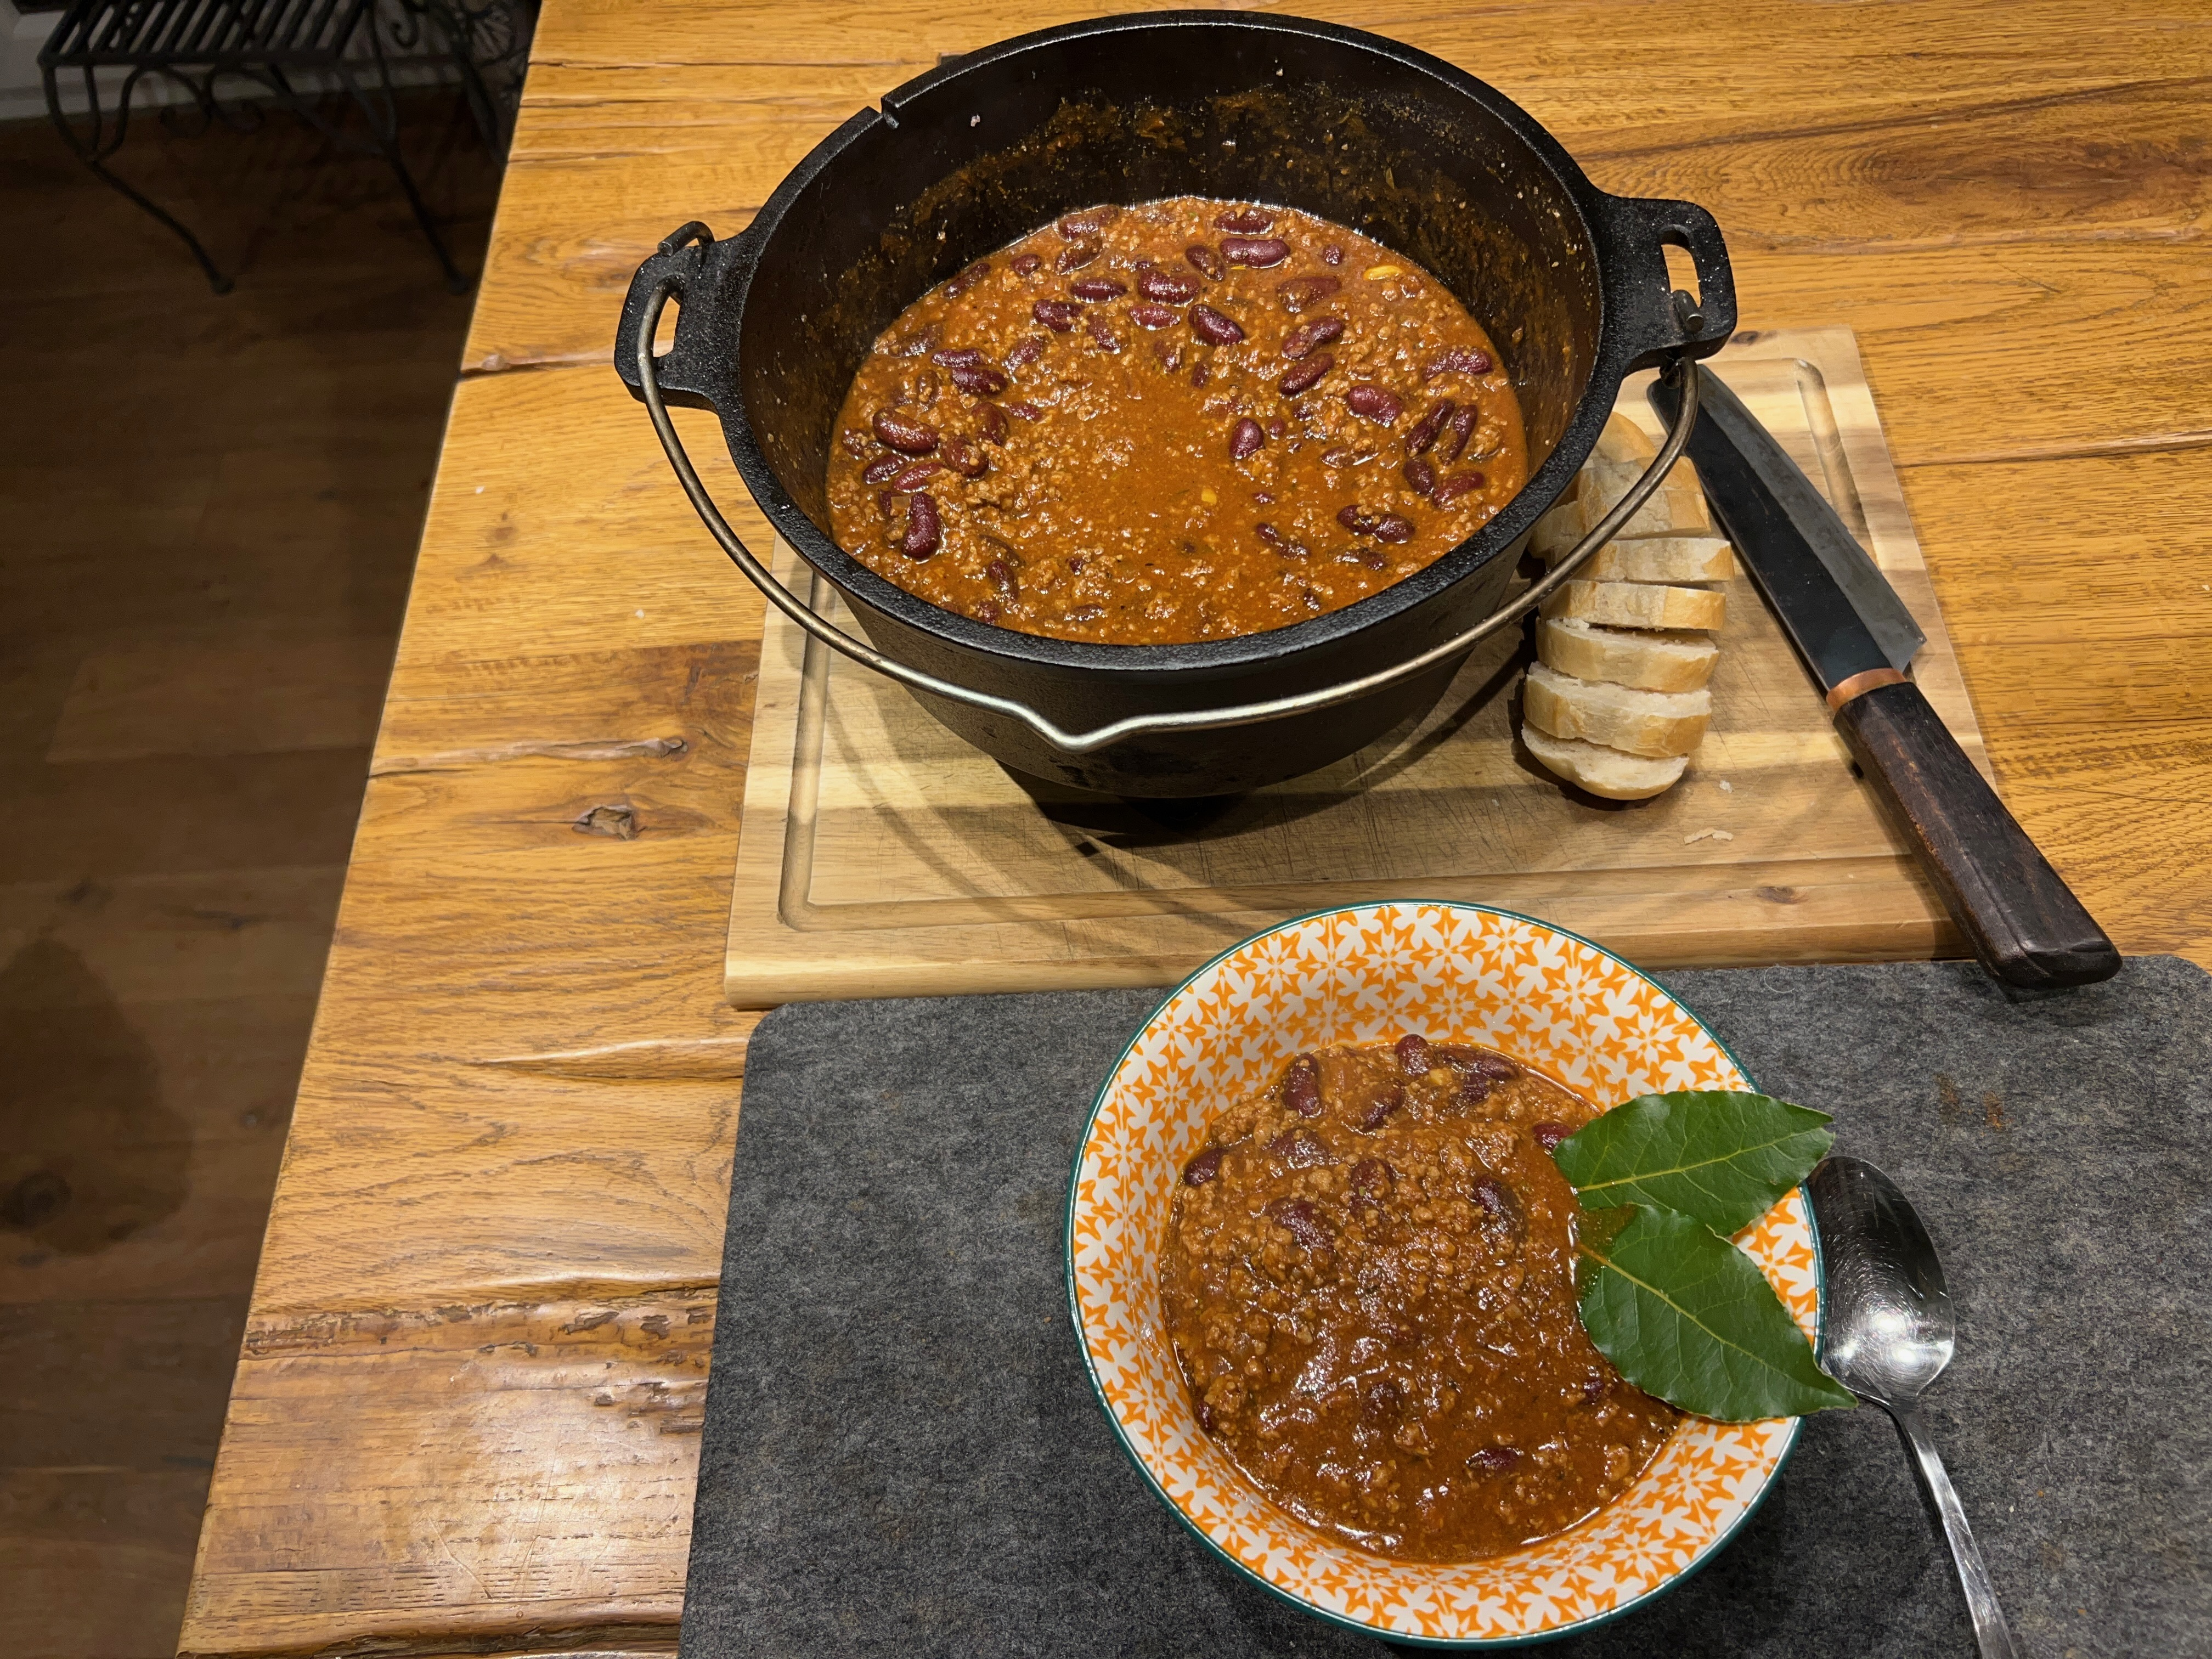
\includegraphics[width=.9\linewidth]{pics/Schwarzes Chili}
		\captionof{figure}{Schwarzes Chili aus dem Dutch oven}
		\label{fig:Schwarzes_Chili}
	\end{minipage}
\end{figure}
\newpage


\subsubsection{Helles Chili}\label{Helles Chili}

\paragraph{Geräte}

\begin{itemize}[noitemsep]
	\item Dutch oven
\end{itemize}

\paragraph{Zutaten}

\begin{itemize}[noitemsep]
	\item  500 g Hühner- oder Putenbrust
	\item 1 Gemüsezwiebel
	\item 1 chinesischer Knoblauch
	\item 1 Dose Mais (400 g)
	\item 2 Dosen Weiße Bohnen (400 g)
	\item 1 Grüne Paprikaschote
	\item 2 cl Veterano Brandy oder Goldener Tequila
	\item 1 EL Berberitze (für die Säure)
	\item 3-5 Lemondrop Chilis (je nach Geschmack)
	\item 50 ml Olivenöl
	\item 50 ml Sonnenblumenöl
	\item 20 g Weiße Schokolade
	\item 1 EL Gekörnte Brühe
	\item 1/2 TL Piment, ganz
	\item 1/2 TL Kardamom
	\item 1 TL geriebener Ingwer
	\item 1/2 TL Koriandersamen
	\item 1 Prise Zimt
	\item Salz \& Pfeffer
	\item 200 ml Wasser
\end{itemize}

\paragraph{Zubereitung}

Piment, Kardamom und Koriandersamen in einer Pfanne anrösten bis Knackgeräusche zu hören sind. Abkühlen lassen und fein mörsern oder in einer Gewürzmühle mahlen. Danach mit den anderen Gewürzen, bis auf Salz und Pfeffer, vermischen und zur Seite stellen.
Die Zwiebeln, die Chilis und den Knoblauch in Würfel schneiden und im Olivenöl andünsten. Zwischenzeitlich die Hühner- oder Putenbrust und die Paprikaschote in Würfel (ca. 1 cm Kantenlänge) schneiden und das Fleisch im Sonnenblumenöl scharf und kurz anbraten.
Die angedünsteten Zutaten zu dem Fleisch geben, nochmals bei starker Hitze rösten um Röststoffe zu entwickeln. Den Tequila oder Brandy zugeben, sobald der Alkohol verkocht ist mit dem Wasser ablöschen. Den Mais, die Berberitze  und den Paprika zugeben, das Ganze 15 Minuten bei mittlerer Hitze ohne Deckel köcheln lassen.  
Die Bohnen und die Gewürze zugeben und alles nochmals 15 Minuten ohne Deckel köcheln lassen. Mit Salz und Pfeffer abschmecken.
Das Chili in einer Schüssel servieren und Weißbrot dazu reichen.
\newpage

\subsection{Rinderrouladen aus dem Dutch oven}

\paragraph{Geräte}

\begin{itemize}[noitemsep]
	\item Dutch oven
\end{itemize}

\paragraph{Zutaten}

\begin{itemize}[noitemsep]
	\item 1- 2 Rouladen pro Person
	\item 1 EL Senf pro Roulade
	\item 1/4 Gewürzgurke pro Roulade (längs geviertelt)
	\item 1/2 kleine Zwiebel Pro Roulade
	\item 1-2 Scheiben Speck oder Bacon pro Roulade
	\item Salz \& Pfeffer
	\item Paprikapulver
	\item etwas Zucker
	\item 1 EL Tomatenmark
	\item 2 EL Öl zum Braten
	\item etwas Wurzelgemüse (nach Geschmack)
	\item Bratensauce
	\item etwas Sahne (oder Saucenbinder)
\end{itemize}

\paragraph{Zubereitung}

Die Rouladen auf einem Schneidebrett aus legen und mit Senf bestreichen, 
mit Salz und Pfeffer würzen. Danach den Speck oder Bacon und 
Zwiebelringe längs auf die Roulade legen. Die geviertelte Gurke quer an 
eine kurze Seite legen und die Roulade um die Gurke aufrollen und mit 
Zahnstochern fixieren.
Die Rouladen mit dem Öl im Dutch oven von allen Seiten dunkelbraun 
anbraten. Dazu soviel Kohle verwenden wie unter den Dutch oven passen. 
Die fertig gebratenen Rouladen zu Seite legen. 
Das Tomatenmark im Dutch anbraten, bitte nicht bis es bitter wird. 
Reichlich Pfeffer, Salz und Paprika, die restlichen Zwiebeln und das 
Wurzelgemüse dazu geben. Dananch mit der Bratensoße auffüllen und die 
dem Bratensatz durch rühren lösen. Die Rouladen in die Soße zurückgeben 
und 2 bis 3 Stunden simmern lassen. Die Rouladen ab un zu drehen und 
dabei kontrollieren ob das Fleisch schon mürbe ist. Ca. 10 Kohlen unter 
dem Feuertopf sollten reichen. Kohlen auf dem Deckel sind nicht 
notwendig.
\newpage

\begin{figure}[htbp]
	\centering
	\begin{minipage}{1\textwidth}
		\centering
		\includegraphics[width=.9\linewidth]{pics/Rinderrouladen}
		\captionof{figure}{Rinderrouladen aus dem Dutch oven}
		\label{fig:Rinderrouladen}
	\end{minipage}
\end{figure}
\newpage

\section{Schwein}

Es gibt deutlich weniger Schweinerassen als Rinderrassen die zum Grillen 
sehr beliebt 
sind. Hier werde ich einige der bedeutendsten Rassen vorstellen. Die 
Schweinerassen  sind sowohl in Gourmet-Kreisen als auch in der 
BBQ-Szene bekannt und beliebt.

\begin{description}
	\item[Das Bunte Bentheimer Schwein] stammt aus der Grafschaft 
	Bentheim im Emsland. Die Rasse wird wieder verstärkt gezüchtet und 
	somit wird die seltene Rasse weiträumiger Verfügbar. Das Fleisch hat 
	eine vergleichbar hohen Fettgehalt, das dadurch sehr schmackhafte 
	Fleisch ist in der gehobenen Gastronomie sehr gefragt.
	\item[Das Duroc] ist durch seine rot-braune Farbe und Schlappohren 
	leicht zu erkennen. Der Ursprung dieser Rasse ist nicht eindeutig 
	geklärt, zu kam sie entweder aus Südamerika mit den Spaniern oder 
	aus Afrika mit dem Umweg über Amerika. Das dunklere reine 
	Duroc-Fleisch enthält mehr intramuskuläres Fett und das schmeckt 
	Ihr auf eurem Teller: Das Fleisch ist feinfaserig, zart und hat einen 
	kräftigen Geschmack
	\item[Das Iberico-Schwein] ist wohl das edelste Schwein, es sind 
	halbwilde Schweine die pfleglos im Freien gehalten werden. Da nicht 
	zugefüttert wird, ernähren sich die Schweine von Eicheln der Stein- 
	und Korkeichen sowie Kräutern. Als Eiweißquellen dienen, 
	Regenwürmer, Käfer, Schnecken. 
	\begin{itemize}[noitemsep]
		\item Jamón Ibérico de Bellota oder Jamón Ibérico terminado en 
		montanera stammt von freilaufenden Schweinen, die ca. 40\% ihres 
		Lebendgewichts durch Eicheln der Steineichen und Korkeichen 
		sowie Kräuter erreicht haben. Die Eicheln sorgen für den nussartigen 
		Geschmack.
		\item Jamón Ibérico de Recebo stammt von Schweinen, denen Eicheln 
		zugefüttert wurden. In dieser Zeit erhöht sich das Anfangsgewicht 
		durch Eicheln und Kräuter um ca. 30\%. Die Endmast erfolgt mit 
		Getreide und Viehfutter.
		\item Der Jamón Ibérico de Pienso (Campo) stammt von Schweinen, 
		die im Stall nur mit Getreide und Viehfutter gemästet wurden.
	\end{itemize}
\end{description}




\subsection{Spare ribs 3-2-1 Methode}
Spare ribs sind ein Bestandteil der "<Holly trinity of BBQ">  oder der 
">Dreifaltigkeit des BBQ">. Die beiden anderen Bestandteile sind Pulled 
Pork und Beef Brisket. 
Es gibt verschiedene Methoden Spare ribs zuzubereiten. Die wohl 
populärste ist die 3-2-1-Methode. Der Name erschließt sich aus der 
Zubereitung. Drei Stunden räuchern, 2 zwei Stunden dämpfen und eine 
Stunde glasieren. Abgeleitet davon gibt es noch die  4-1-1-Methode und 
die 5-0-1-Methode. Wie bei der 3-2-1-Methode bedeutet die erste Ziffer 
die Zeit in Stunden des Räucherns, die zweite Ziffer die Zeit in Stunden 
des Dämpfens und last but not least die dritte Ziffer die des Glasieren 
ebenfalls in Stunden.  
Bei der 3-2-1 werden die ribs so mürbe, dass sie fast vom Knochen fallen, 
im Jargon heißt es "> Falling of the bones"<. Bei der 4-1-1 Methode löst 
sich da Fleisch leicht vom Knochen hat aber noch Biss, während die 5-0-1 
Methode den meisten Rauchgeschmack mitbringt und deutlich bissfester 
ist als die anderen Methoden.

Als weitere Methoden sind

\begin{itemize}[noitemsep]
	\item Vorgaren im Backofen, scharf Angrillen und Glasieren
	\item Sous vide Garen, scharf Angrillen und Glasieren
	\item Schmoren im Dutch oven, scharf Angrillen und Glasieren
\end{itemize}
zu nennen.
\newline

\paragraph{Geräte}

\begin{itemize}[noitemsep]
	\item Kugelgrill
	\item Water Smoker
 	\item Gasgrill (min. 3 Brenner)
	\item Kamado Grill (Keramik Grill)
\end{itemize}

Die Handhabung der Geräte wird in Kapitel\ref{Chapter1} erklärt

\paragraph{Zutaten für 4 Personen}

\begin{itemize}[noitemsep]
	\item 2,0 bis 2,4 kg Spare ribs St. Louis Cut oder Baby Back Ribs
	\item Kansas City Rib Rub (Rezept siehe Kapitel~\ref{Chapter6} 
	\vref{Kansas})
\end{itemize}

Zutaten für die Glasur:
\begin{itemize}[noitemsep]
	\item 200 g Himbeermarmelade
	\item 100 ml Apfelsaft
	\item 1 EL Balsamico Essig
	\item Salz
	\item Pfeffer	
\end{itemize}

Vorbereitung: Bei dem Kugelgrill und dem Water Smoker Junks auf die Holzkohle geben. Hier Hickory oder Apfel.
Bei dem Kamado Grill Räucherchips verwenden, die uneingeweicht auf die Holzkohle gegeben werden.
Bei dem Gasgrill Räucherpellets oder -chips in Wasser einweichen und in 
eine Räucherbox geben und diese auf den Gasbrenner stellen. Hier 
ebenfalls Hickory oder Apfel

\paragraph{Zubereitung der Glasur:}

Die Marmelade durch ein Sieb streichen (um die Kerne zu entfernen) 
Danach alle Zutaten in einem Topf vermengen und ca. 5 Minuten köcheln.

\paragraph{Zubereitung der Spare ribs:}

Silberhaut von den Spareribs (auf der Knochenseite) entfernen.
Die Spareribs auf jeder Seite gut mit dem Kansas City Rib Rub einreiben, 
mind. 30 Minuten ruhen lassen (besser über Nacht).
Die Ribs in Rippchenhalter und auf den Rost des vorbereiteten 
Geräts stellen.
Die Ribs bei 120°C für 3 Stunden räuchern. Danach die Ribs in eine 
Schale mit ein wenig Apfelsaft legen, die Schale mit Alufolie dicht 
abdecken. Den Grill auf 140°C bis 150°C aufheizen und die Ribs für 2 
Stunden bei 150°C dämpfen.
Nach 2 Stunden die Rippchen aus Schale nehmen und mit der Marinade 
einpinseln. Eine weitere Stunde glasieren, evtl. nach 30 Minuten erneut 
Marinade aufbringen.
Die Rippchen sind durch wenn man sie auf der einen Seite mit der 
Grillzange aufnimmt und die Rippchen durchhängen und das Fleisch 
einreißt. 
\newpage
\begin{figure}[htbp]
			\centering
		\begin{minipage}{1\textwidth}
		\centering
		\includegraphics[width=1\linewidth]{pics/SpareRibs1}
		\captionof{figure}{Spare ribs}
		\label{fig:Spare}
		\end{minipage}
\end{figure}
\newpage

\subsection{Pulled pork, low \& slow}
Pulled Pork gehört ebenso wie die Spare ribs und das Beef brisket zu 
dem "<Holly trinity of BBQ">. Wie beim Beef brisket ist auch hier einen 
Menge Geduld gefragt. Denn bekanntlich ist Geduld der beste Koch. Das 
Pulled pork ist ein Klassiker und wird traditionell in Burger buns serviert. Allerdings ist 
es kein Sakrileg wenn das Pulled Pork mit Colslaw und baked beans oder 
einem lauwarmen Gemüsesalat serviert wird.

\paragraph{Geräte}

\begin{itemize}[noitemsep]
	\item Kugelgrill
	\item Water Smoker//
 	\item Gasgrill (min. 3 Brenner)//
	\item Kamado Grill (Kramikgrill)
\end{itemize}

Die Handhabung der Geräte wird in Kapitel\ref{Chapter1} erklärt

\paragraph{Zutaten für 10 Personen:}

\begin{itemize}[noitemsep]
	\item 5 kg Boston Butt
	\item BBQ-Rub, z.B. Magic dust Rub (Rezept siehe 
	Kapitel~\ref{Chapter6} \vref{Magic})
\end{itemize}

\paragraph{Zutaten für das Dämpfen:}

\begin{itemize}[noitemsep]
	\item 100 ml Apfelsaft
\end{itemize}

Vorbereitung: Bei dem Kugelgrill und dem Water Smoker Junks auf die Holzkohle geben. Hier 
Hickory oder Apfel.
Bei dem Kamado Grill Räucherchips verwenden, die uneingeweicht auf die Holzkohle gegeben 
werden.
Bei dem Gasgrill Räucherpellets oder -chips in Wasser einweichen und in 
eine Räucherbox geben und diese auf den Gasbrenner stellen. Hier 
ebenfalls Hickory oder Apfel

Der typische amerikanische Cut für Pulled pork ist der Boston Butt. Dabei 
handelt es sich um Schweinenacken an den noch ein Stück von der 
Schulter  inklusive komplettes Schulterblatt anhängt, das so genannte 
Horn.
Das Boston Butt wird großzügig mit dem gewählten Rub einreiben und 30 
Minuten ruhen lassen (besser über Nacht) Die Grills bzw. Water Smoker 
auf ca. 110°C einstellen, das Fleisch auf die indirekte Zone legen und für 
12 Stunden räuchern. Danach das Fleisch vom Grill nehmen und in eine 
Edelstahl- oder Auflaufform legen. Den Apfelsaft dazu geben und mit 
Aluminiumfolie dicht abdecken. Das Fleisch dann bei 135°C ca. 3 Stunden 
dämpfen. Nach dem Dämpfen muss das Fleisch eine Kerntemperatur von 
95°C erreicht haben. Das Fleisch wird dann zum Ruhen für eine 1 Stunde 
in eine Thermobox verfrachtet. Dieser Schritt ist wichtig, damit sich das
Fleisch entspannen kann und der Saft sich schön verteilt. Nach dem 
Ruhen das Fleisch nochmals für 30 Minuten auf den Grill legen, damit 
seine Kruste bildet.

Nun den Knochen und die Sehnen entfernen und das Fleisch mit den 
Händen oder Gabeln rupfen wie in Abbildung~\vref{fig:PulledPork} zu 
sehen, danach als Pulled Pork Burger oder auf dem Teller mit Beilagen 
servieren.
\newpage
\begin{figure}[htbp]
		\centering
		\begin{minipage}{1\textwidth}
		\centering
		\includegraphics[width=1\linewidth]{pics/Pulled_Pork}
		\captionof{figure}{Pulled Pork}
		\label{fig:PulledPork}
	\end{minipage}
\end{figure}
Von Thogru - Eigenes Werk\\
CC BY-SA 3.0, https://creativecommons.org/licenses/by-sa/3.0
\newpage

\section{Lamm}

Lammfleisch stammt von jungen Schafen, die nicht älter als ein Jahr sind. Es ist besonders zart 
und mild im Geschmack. 
Wird das Fleisch von einem Schaf, das älter als ein Jahr, aber jünger als zwei Jahre ist, 
geschlachtet, spricht man von 
Hammelfleisch. Schaffleisch hingegen kommt von Schafen, die älter als zwei Jahre sind. Je älter 
das Tier, desto intensiver
und kräftiger wird der Geschmack des Fleisches.

Lammfleisch hat eine hell- bis dunkelrote Farbe und zeichnet sich oft durch eine feine 
Marmorierung aus. Je nach Cut kann
es mehr oder weniger Fett enthalten, was den Geschmack und die Zartheit des Fleisches 
beeinflusst. Geschmacklich ist
Lammfleisch mild und leicht süßlich, oft mit einer subtilen Note von Kräutern und Gräsern, die 
die Tiere während ihres Leben
gefressen haben. Hochwertiges Lammfleisch hat keinen strengen Geschmack, sondern ist zart 
und saftig.

\subsection{Uwe's Irish Stew}

Irish Stew ist ein Eintopf der in Irland ein Nationalgericht ist. Traditionell wir dieser Eintopf mit 
Lammfleisch zubereitet. Es
gibt allerdings eine Menge Rezepte, die mit alternativen Fleischsorten (z.B. Rind und/ oder 
Schwein) zubereitet werden. Das folgende Rezept
gilt auch für ein Irish Stew das nicht mit Lammfleisch zubereitet wird. Bei der Auswahl der 
Gemüse gilt das Motto ">Feel free"<, alles
was schmeckt ist erlaubt. Es gibt nicht das Rezept, sondern eine Menge Rezepte von Haushalt 
zu Haushalt verschieden. Ich werde euch
meine Interpretation des Irish Stew vorstellen, siehe Abbildung~\vref{fig:Irish_Stew}.

\paragraph{Geräte}

\begin{itemize}[noitemsep]
	\item Dutch oven (Hitzequelle nach Wahl)
\end{itemize}

\paragraph{Zutaten für 4 Personen}

\begin{itemize}[noitemsep]
	\item 1 kg Lammfleisch (aus der Keule oder Schulter)
	\item 1 mittelgroße Zwiebel
	\item 2 Zehen Knoblauch
	\item 150 g Petersilienwurzel
	\item 150 frischer Fenchel
	\item 150 g Staudensellerie
	\item 300 g Karotten
	\item 300 ml Dunkles Weizenbier
	\item 1000 ml Brühe 
	\item 2 Lorbeerblätter
	\item 1 ganze Nelke
	\item 3 Wacholderbeeren
	\item 2 Pimentkerne
	\item 1/2 TL Fenchelsamen
	\item Salz \& Pfeffer
	\item Butterschmalz zum anbraten des Fleisches
\end{itemize}

\paragraph{Zubereitung}

Fleisch und Gemüse in mundgerechte Stücke schneiden, Knoblauch feinhacken. 
Fleisch im Dutsch oven in Portionen scharf anbraten bis sich Röststoffe bilden. Das Fleisch 
aus dem Dutch oven nehmen und die Karotten, den Fenchel, den Staudensellerie und die 
Petersilienwurzeln anbraten. Sobald sich Röststoffe bilden die Zwiebeln und den Knoblauch 
dazu geben. Wenn die Zwiebeln Farbe annehmen das ganze mit dem Bier ablöschen. Das 
Fleisch und die Gewürze hinzugeben und mit der Brühe auffüllen. Das ganze bei mittlere Hitze 
ca. 2 Stunden
schmoren lassen. Ich lasse das Irish Stew immer abkühlen und wärme es am nächsten Tag auf,
aus diesem Grund gare ich die Kartoffeln nicht im Irish Stew mit, sondern frisch vor den 
Servieren. 
Vor dem Servieren nochmals mit Salz und Pfeffer abschmecken.

\begin{figure}[htbp]
	\centering
	\begin{minipage}{1\textwidth}
		\centering
		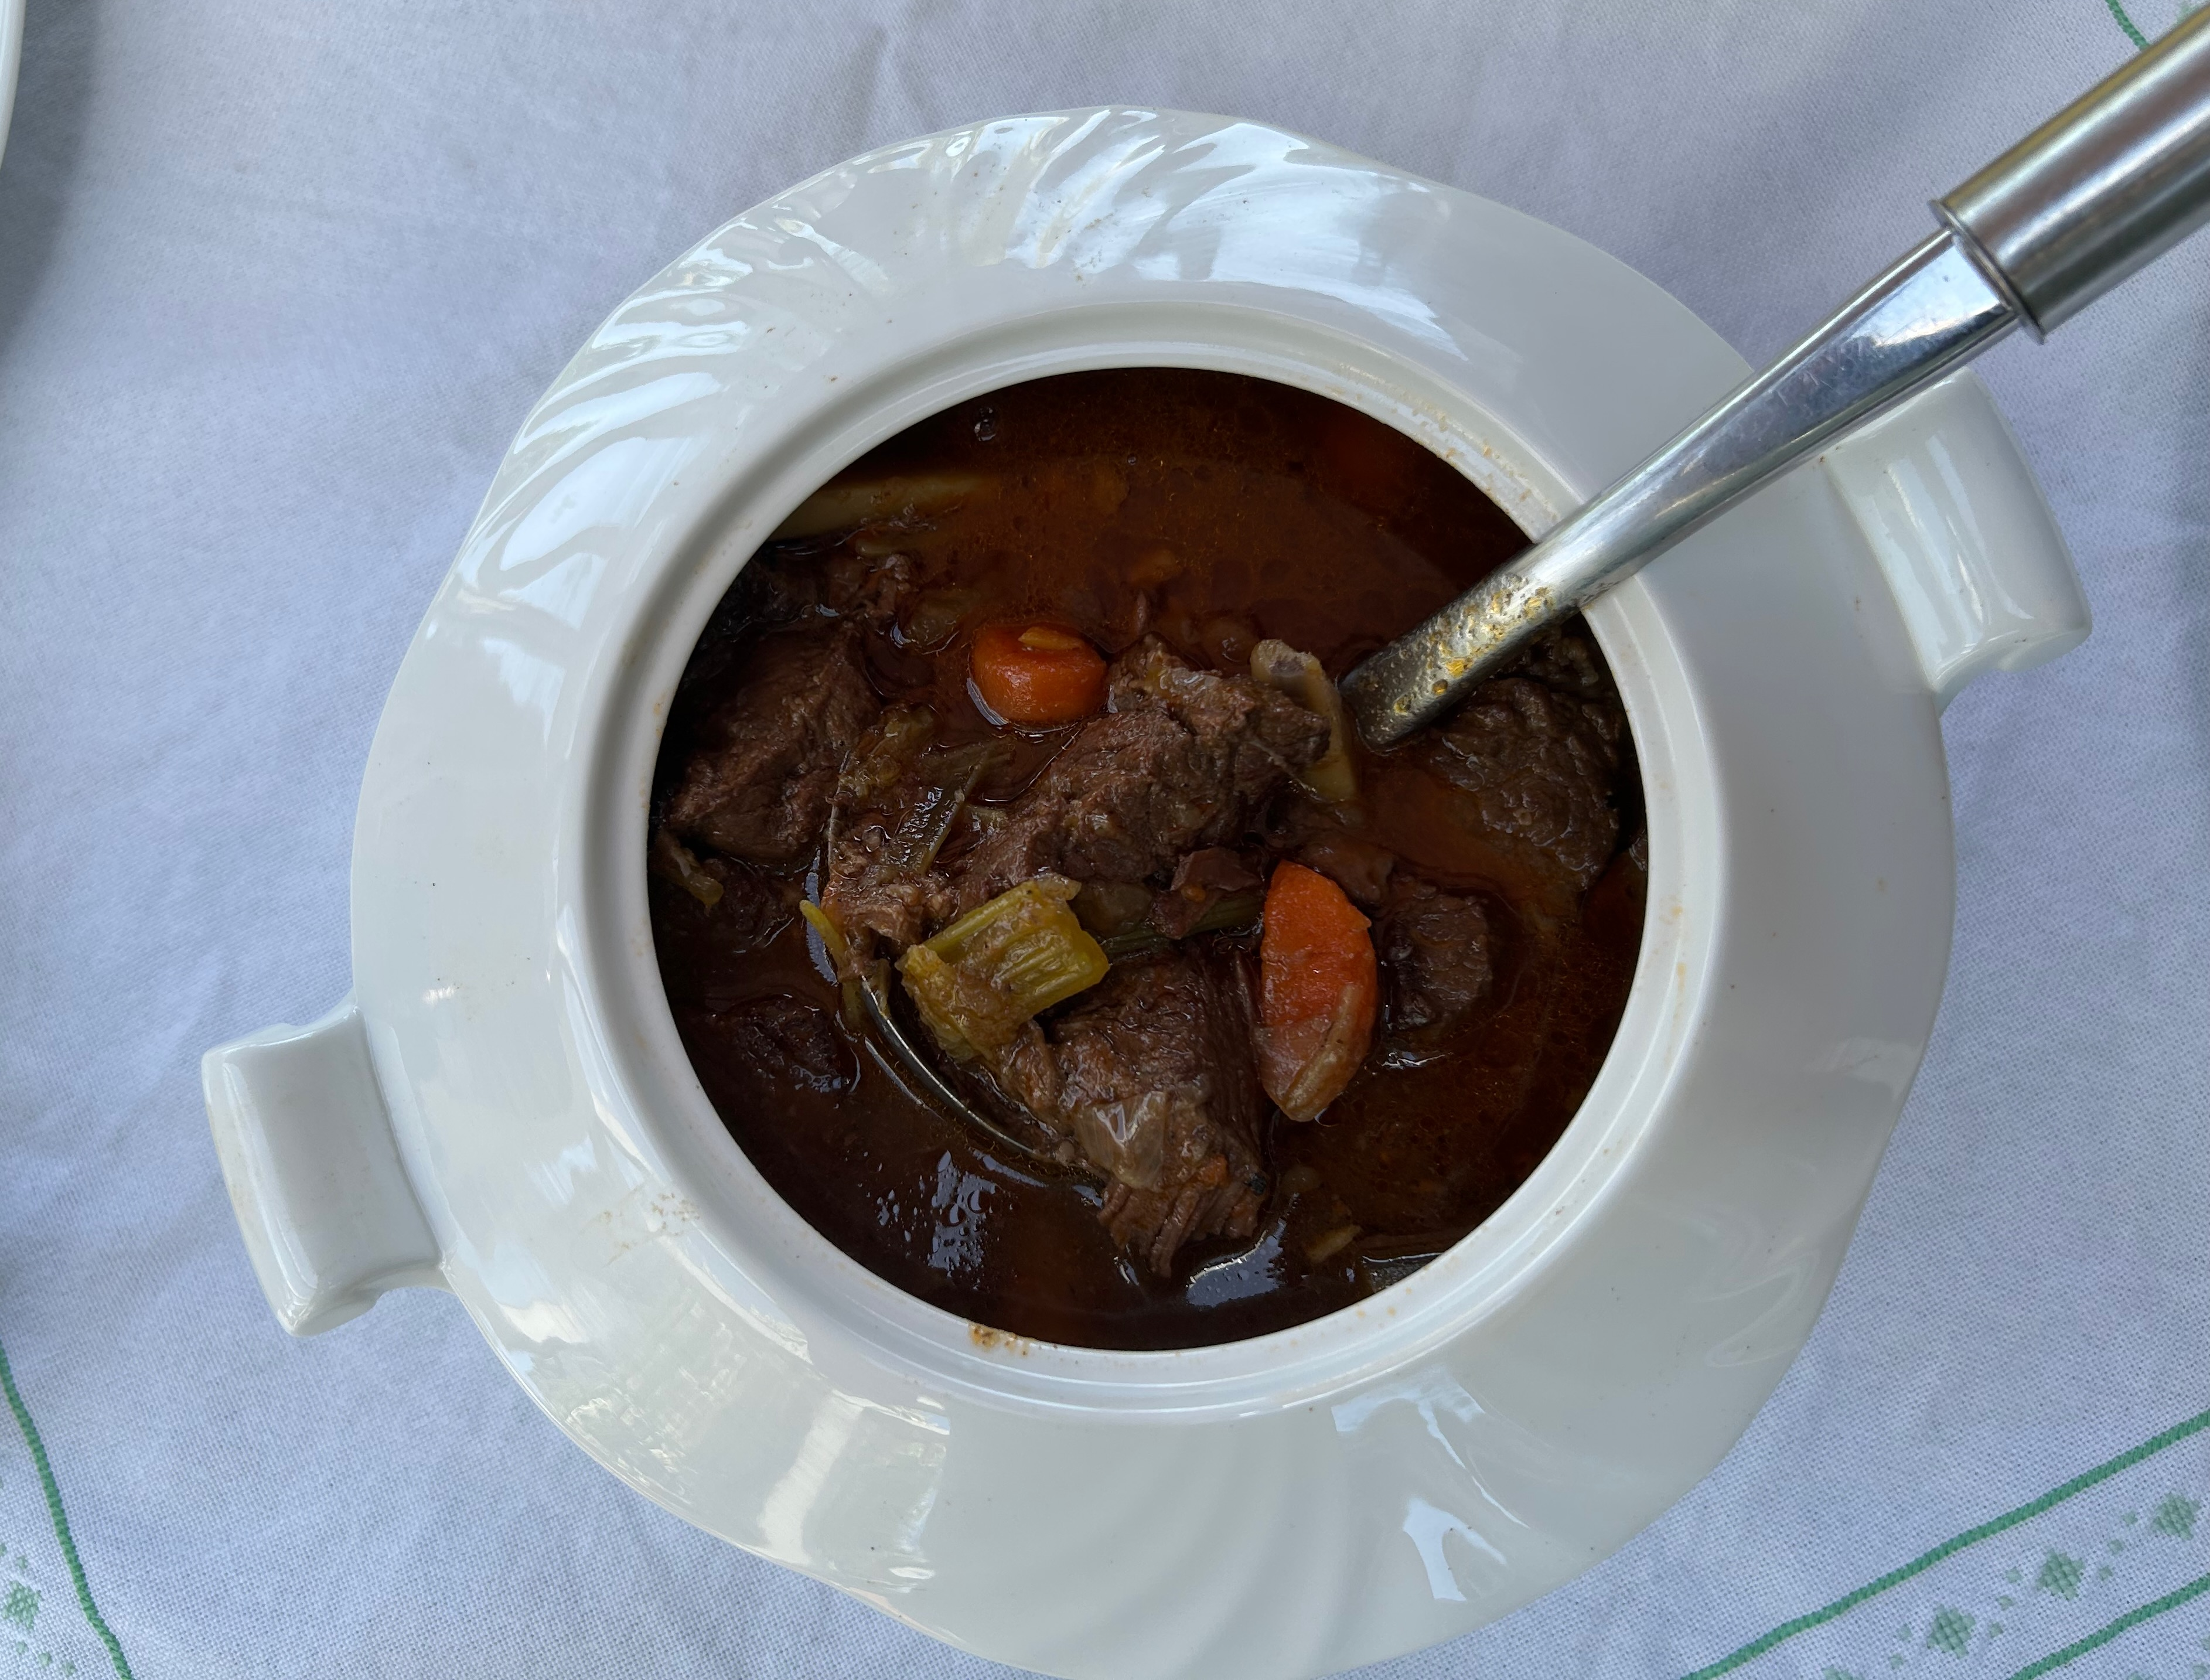
\includegraphics[width=1\linewidth]{pics/Irish_Stew}
		\captionof{figure}{Irish Stew}
		\label{fig:Irish_Stew}
	\end{minipage}
\end{figure}
\newpage


\section{Geflügel}

\subsection{Road Killed Chicken}

\paragraph{Geräte:}

\begin{itemize}[noitemsep]
	\item Kugelgrill
 	\item Gasgrill (min. 3 Brenner)
	\item Kamado Grill (Keramikgrill)
\end{itemize}

\paragraph{Zutaten für das Road Killed Chicken}

\begin{itemize}[noitemsep]
	\item Label rouge franz. Maishuhn
	\item Chicken Rub (Rezept siehe Kapitel~\ref{Chapter6} \vref{Chicken})
\end{itemize}

Wie wird das Hähnchen für „Road Killed Chicken“ vorbereitet?

Das ist wirklich einfach: Ihr legt das Hühnchen auf die Brustseite und 
schneidet mit einem Sägemesser oder einer Geflügelschere links und 
rechts neben dem Rückgrat komplett von oben nach unten durch. Den 
Knochenstrang könnt ihr dann einfach entnehmen (und möglicherweise 
mit anderen Fleischabschnitten zu Hühnerbrühe kochen). Wenn ihr das 
Huhn nun auseinandergeklappt auf die Innenseite legt, ist es ziemlich 
flach. Drückt gegebenenfalls nochmal fest mit der Hand aufs Brustbein, 
um es noch flacher zu machen. Der Vorteil dieser Methode ist, dass das 
Huhn gleichmäßig flach ist und daher schnell gart. Dadurch bleibt das 
Huhn schön saftig mit krosser Haut wie in 
Abbildung~\vref{fig:RoadKilledChicken}.

Den Grill (egal welchen Ihr einsetzen wollt) auf 180°C indirekte Hitze 
einstellen.
Das Huhn mit der Brustseite nach oben auf den Grill legen und bis zu 
einer Temperatur in der Keule vom 90°C grillen. Das Huhn vom Grill 
nehmen mit Salaten und Baguette servieren, lecker.
\newpage

\begin{figure}[htbp]
	\centering
	\begin{minipage}{1\textwidth}
		\centering
		\includegraphics[width=1\linewidth]{pics/Platthuhn_Teller}
		\captionof{figure}{Road Killed Chicken}
		\label{fig:RoadKilledChicken}
	\end{minipage}
\end{figure}
\newpage

\subsection{Buffalo (Chicken) Wings}
Die Buffalo Wings wurden in der Anchor Bar in Buffalo, New York in den 60 
Jahren das erste mal 
zubereitet. Die Wings wurden anfänglich 
noch als Snacks gereicht. Fanden aber mit wachsender Beliebheit schließlich 
den Weg auf die 
Speisekarte. Durch das entstehen der 
Sportsbars in denen die Wings serviert wurden fanden sie Verbreitung in den 
USA. Die Buffalo 
Wings sind seither untrennbar mit Football 
verbunden, ähnlich wie Hot Dogs mit Baseball. Durch diverse Fast Food-Ketten 
fanden sie bald 
weltweit Beachtung.

Die originalen Buffalo Wings wurden frittiert und danach in einer roten Chilisauce 
geschwenkt. 
Meistens wurde dafür Frank's Red Hot 
Sauce als Basis verwendet und mit Butter und weiteren Zutaten veredelt.

Ich stelle euch meine Interpretation der Buffalo Wings vor. 
Inspiriert von Michi von "`Einfach Grillen"' werde ich die Wings auf dem Grill 
unter Zugabe 
von Rauch zubereiten. 

Ich stelle euch außerdem noch drei Arten der Zubereitung der Buffalo Wings 
Sauce vor.

Lasst euch überraschen. Mo und ich halten diese Wings für the best Chicken 
Wings ever.


\paragraph{Geräte:}

\begin{itemize}[noitemsep]
	\item Kugelgrill
	\item Gasgrill
	\item Kamado Grill (Keramikgrill)
\end{itemize}

\paragraph{Zutaten für 2 Personen}

\begin{itemize}[noitemsep]
	\item 2 kg Hühnerflügel (bekommt man in der Regel ohne Spitzen, sollten die 
	Spitzen noch 
	dran sein, bitte entfernen)
	\item 12-15 g Salz
	\item Pfeffer
	\item 1 Päckchen Backpulver (1 je nach Hersteller 15 g bis 17 g)
	\item 1TL Cayennepfeffer
	\item 1,5 gestrichener TL Brauner Rohrzucker
\end{itemize}

Die Hühnerflügel werden in Flat und Drumstick geteilt, in dem sie am Gelenk 
auseinander ge
schnitten werden. Danach werden alle Teile 
trocken getupft (bitte nicht abwaschen) und in eine Schüssel gegeben. Die 
Gewürzmischung 
wird über die Wings gestreut und 
einmassiert. Diese werden dann auf einem Backblech ausgelegt und gekühlt. 
Durch das im Backpulver enthaltene Natron wird die Haut schön trocken, das ist 
die 
Voraussetzung, dass die Wings schön 
knusprig werden.

Den Grill für direkte und indirekte Hitze Vorbereiten und auf ca. 180°C einstellen. 
Dabei ist es 
egal ob Gas-, Holzkohle- oder Keramikgrill. 
Pellets, Chips oder Chunks zum Räuchern bereitstellen. Zu dem Gericht passen 
Buche, Apfel- 
oder Kirsche. Ich persönlich nehme die die 
Whiskey Wood Chips von Napoleon, diese haben ein unglaubliches Aroma.


Die Wings werden über der direkten Hitze scharf angegrillt und danach auf die 
indirekte Zone 
gelegt. Die Wings werden nun  ca. 40 
Minuten auf der indirekten Hitze gegrillt, bitte nicht den Rauch vergessen. 
Während dieser Zeit 
den Deckel bitte nicht lüften, ganz nach 
dem Motto "`if you looking, you ain't cooking"'. Nach 40 Minuten sollte sich das 
Fleisch leicht 
von den Knochen lösen lassen und die 
Wings sehr knusprig sein.

Während die Wings auf den Grill liegen widmen wir uns der Sauce.

Ich versprach euch drei Varianten:

\paragraph{Zutaten Sauce Variante 1}

\begin{itemize}[noitemsep]
	\item ca. 300 ml Frank's Red Hot Wings Sauce
\end{itemize}

Die Sauce im einem Topf erwärmen.

\paragraph{Zutaten Sauce Variante 2}

\begin{itemize}[noitemsep]
	\item 150 g Butter
	\item 2 EL Worcester Sauce
	\item 1 Zehe Knoblauch
	\item ca. 300 ml Frank's Red Hot Sauce
	\item 3 EL Weißweinessig
	\item 1 TL Cayennepfeffer
	\item 2 EL Paprikapulver, süß
	\item 1 Chili (optional)
\end{itemize}

\paragraph{Zutaten Sauce Variante 3}

\begin{itemize}[noitemsep]
	\item 16 Cayenne Chili
	\item 2 Habanero Red
	\item 380 ml Weißweinessig
	\item 2 Zehen Knoblauch
	\item 1 TL Salz
	\item 1 TL Knoblauchpulver
	\item 1 TL geräuchertes Paprikapulver
\end{itemize}

Buffalo Wings Sauce:

\begin{itemize}[noitemsep]
	\item 150 g Butter
	\item 1 EL Worcester Sauce
	\item 1 Zehe Knoblauch 
	\item 3 EL Weißweinessig
	\item 1 TL Kaschmir Chili-Pulver
	\item 1 EL Paprikapulver, süß
	\item 1 Chili (optional)
\end{itemize}

Den Strunk des Habanero und der Cayenne Chilis entfernen und die Schoten 
halbieren. Die Chilis mit den übrigen Zutaten 15 Minuten 
köcheln, mit dem Stabmixer pürieren und durch ein Sieb streichen. Diese Sauce 
mit den weiteren Zutaten zur Buffalo Wings Sauce 
weiterverarbeiten und erwärmen.

Die gegrillten Chicken Wings in der erwärmten Sauce (Variante 1 oder 2 oder 3) 
schwenken, nochmals auf den Grill legen, bis 
die Sauce angetrocknet ist. Die Wings anrichten und die übrige Sauce dazu 
reichen siehe Abbildung~\vref{fig:BuffaloWings}.

In einer Blindverkostung von 10 Familienmitgliedern wurde die Variante 3 mit 10 
von 10 Stimmen als beste Sauce befunden. Dafür danke ich 
herzlichst.                    
\newpage

\begin{figure}[htbp]
	\centering
	\begin{minipage}{1\textwidth}
		\centering
		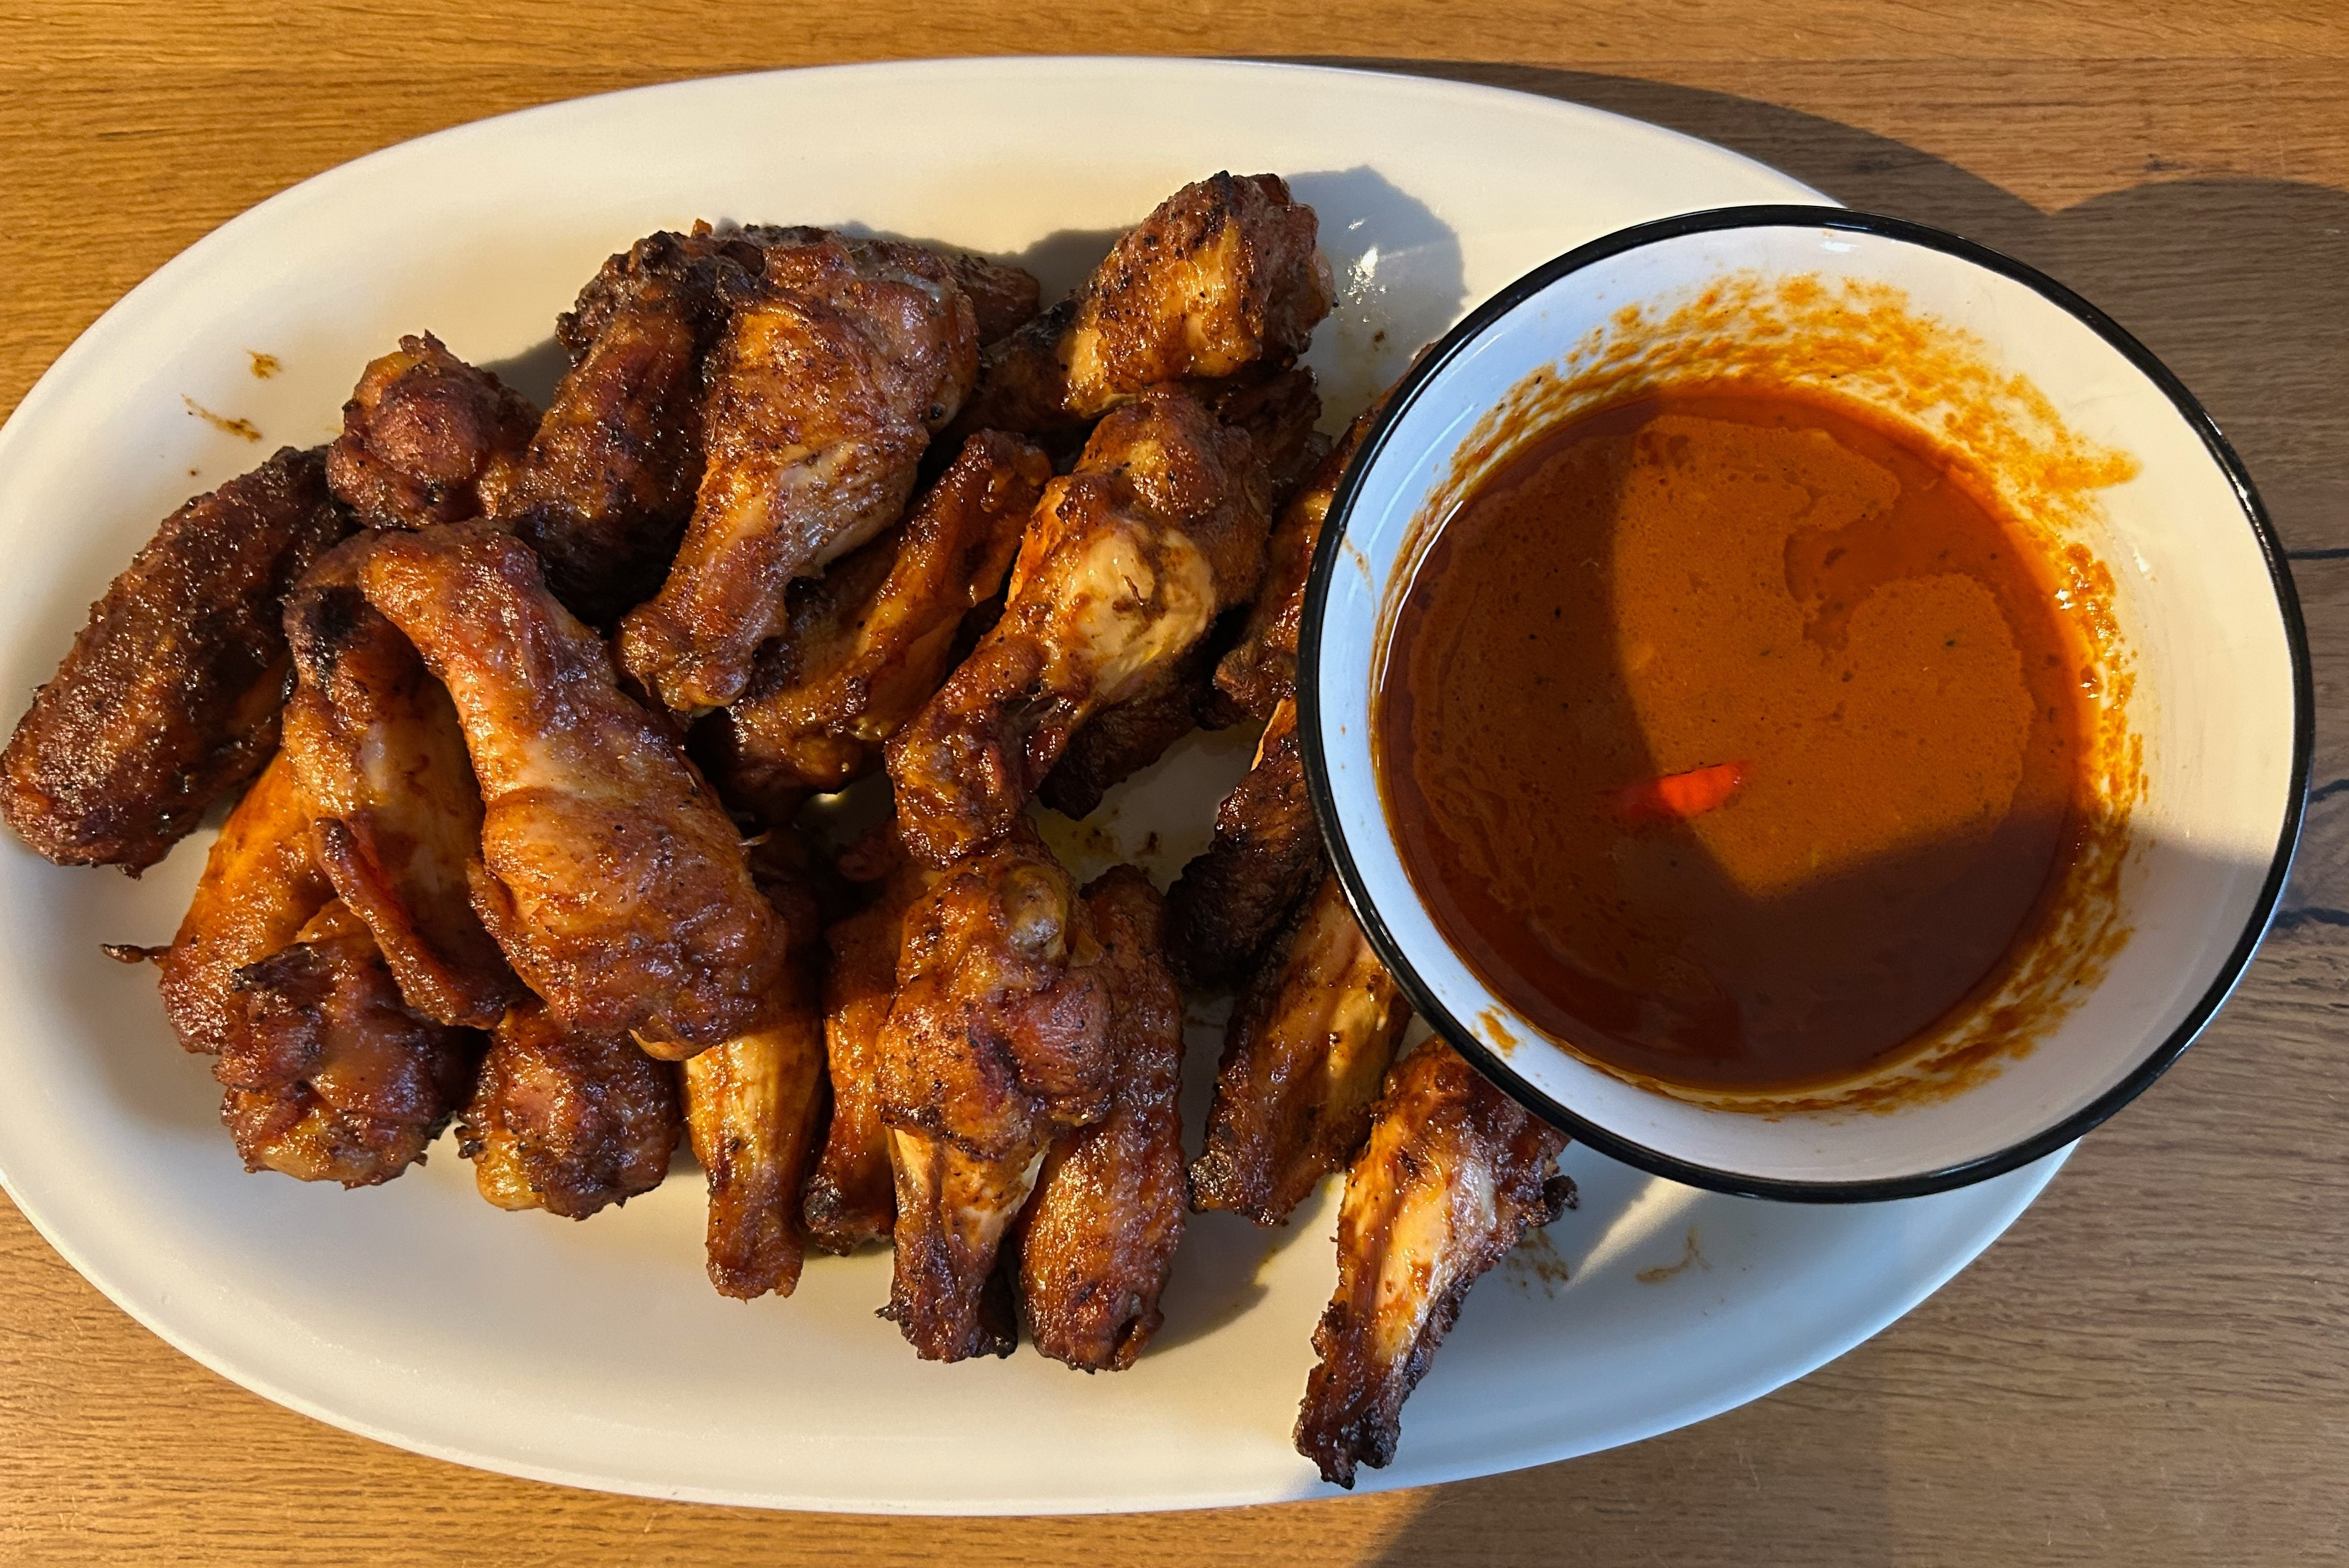
\includegraphics[width=.9\linewidth]{pics/Buffalo_Wings}
		\captionof{figure}{Buffalo Chicken Wings}
		\label{fig:BuffaloWings}
	\end{minipage}
\end{figure}
\newpage



\section{Fisch}

\subsection{Sardinen vom Grill}

\paragraph{Geräte}

\begin{itemize}[noitemsep]
	\item Kugelgrill
	\item Kamado Grill
	\item Gasgrill
\end{itemize}

\paragraph{Zutaten}

\begin{itemize}[noitemsep]
	\item Sardinen, ausgenommen
	\item Salz \& Pfeffer
	\item Eine Zitronenscheibe pro Sardine
\end{itemize}

\paragraph{Zubereitung}

Den Gasgrill auf ca. 200°C vorheizen. Den Rost mit Trennspray einsprühen,  beim Einsprühen gibt es Stichflammen, da die Brenner eingeschaltet sind. Die Sardinen salzen und ca. eine Stunde liegen lassen. Danach die Sardinen auf den Grill legen und von jeder Seite ca. 3 Minuten, je nach Größe,  grillen. 

\begin{figure}[htbp]
	\centering
	\begin{minipage}{1\textwidth}
		\centering
		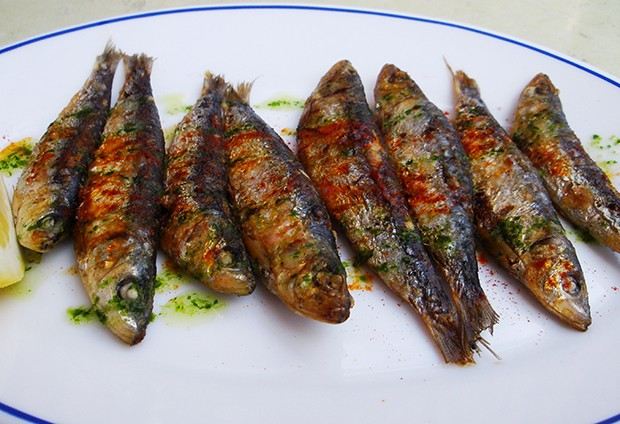
\includegraphics[width=.9\linewidth]{pics/Gegrillte_Sardinen}
		\captionof{figure}{Gegrillte Sardinen}
		\label{fig:Gegrillte_Sardinen}
	\end{minipage}
\end{figure}
\newpage

\subsection{Dorade Royal im Kartoffelbett}

\paragraph{Geräte}

\begin{itemize}[noitemsep]
	\item Gasgrill
\end{itemize}

\paragraph{Zutaten}

\begin{itemize}[noitemsep]
	\item 1 Dorade Royal pro Person
	
\end{itemize}

\paragraph{Zubereitung}

\subsection{Spanische Fischsuppe}

\paragraph{Geräte}


\paragraph{Zutaten}

\paragraph{Zubereitung}

\section{Meeresfrüchte}

\paragraph{Geräte}

\paragraph{Zutaten}

\paragraph{Zubereitung}


\subsection{Gegrillte Garnelen}

\paragraph{Gräte}

\paragraph{Zutaten}

\paragraph{Zubereitung}


\subsection{Ingwer-Garnelen vom Grill}

\paragraph{Geräte}

\paragraph{Zutaten}

\paragraph{Zubereitung}


\subsection{Pulpotentakeln vom Grill}

\paragraph{Geräte}

\paragraph{Zutaten}

\paragraph{Zubereitung}


\subsection{Dreierlei Muscheln von der Plancha}

\paragraph{Geräte}

\paragraph{Zutaten}

\paragraph{Zubereitung}